% *************************************************************************
% *    IWI Hamburg / Prof. Dr. Stefan Voß
% *    Thesis / Dissertation Latex Template                                        
% *    
% *    Author: Leonard Heilig <leonard.heilig@uni-hamburg.de>
% *   
% *    Note: some parts of this template are based on the VSIS template
% *              of Michael von Riegen <riegen@informatik.uni-hamburg.de>
% *   
% *************************************************************************
\RequirePackage{scrlfile}
\ReplacePackage{scrpage2}{scrlayer-scrpage}
\documentclass[
      paper=a4,
      12pt,
      twoside=false,
      openright,
]{scrbook}



% DEFINE THESIS SETTINGS
% Bitte füllen Sie die folgenden Daten vollständig aus
\newcommand\myName{Daniel Braun}
\newcommand\myAddress{Curt-Bär-Weg 129, 21035 Hamburg}
\newcommand\myEmail{Daniel.Braun-2@studium.uni-hamburg.de}
\newcommand\myKeywords{Blockchain-Technologie, Bitcoin, Ethereum, Smart Contract, Online Advertising, Programmatic Advertising} % Optional
\newcommand\myMatNr{6922337}
\newcommand\myTitle{Blockchain-Technologie im Online Advertising}
\newcommand\myShortTitleForHeader{Blockchain im Online Advertising}
\newcommand\thesisType{Bachelorarbeit}
\newcommand\faculty{MIN-Fakultät} % z.B. MIN-Fakultät
\newcommand\fachbereich{} % Optional: z.B. Fachbereich Informatik
\newcommand\courseOfStudies{B.Sc. Wirtschaftsinformatik}
\newcommand\supervisor{Michael Palk}
\newcommand\primaryReferee{Prof. Dr. Stefan Voß}
\newcommand\primaryRefereeInst{Institut für Wirtschaftsinformatik}
\newcommand\secondaryReferee{Dr. Kai Brüssau}
\newcommand\secondaryRefereeInst{Institut für Wirtschaftsinformatik}
\newcommand\optionalQuote{} % shown after title page

\title{\mytitle}
\author{\myName \\ \texttt{\myEmail}}

% IMPORT PACKAGES AND SETTINGS
\usepackage{settings}
\usepackage{longtable}
\usepackage{float}
\usepackage{listings}



\renewcommand{\lstlistingname}{Programmcode}
\renewcommand{\lstlistlistingname}{\lstlistingname}

% ************ DOCUMENT BEGINS

\begin{document}

    % CHOOSE "ngerman" or "english"
    \selectlanguage{ngerman}
    
    % Please change this part to _titlepage_en for the English version
    % *************************************************************************
% *    Thesis / Dissertation Latex Template                                        
% *    
% *    Author: Leonard Heilig <leonard.heilig@uni-hamburg.de>
% *   
% *    Note: some parts of this template are based on the VSIS template
% *              of Michael von Riegen <riegen@informatik.uni-hamburg.de>
% *   
% *************************************************************************

\begin{titlepage}

% START PAGE: -1
\setcounter{page}{-1}    

\begin{figure}[h]
    
    \begin{flushleft}
   
    \end{flushleft}
    \hspace{-40px}
    \noindent\begin{minipage}[t][0px][b]{0.3\textwidth}
    	%\noindent
\includegraphics[width=8cm,clip]{images/up-uhh-logo-u-2010-u-png}
    	\noindent
\includegraphics[scale=0.3]{images/UHH-Logo_2010_Farbe_CMYK.pdf}
    \end{minipage}
    \hspace{50px}
    \begin{flushright}
    	  
    	 \begin{minipage}[t][-70px][b]{0.38\textwidth}
    	 	\begin{flushright}
    	 	\sffamily{
    	 		%{\small \textbf{Institut für Wirtschaftsinformatik} } \\
    	 		%\small Prof. Dr. Stefan Voß \\
    	 	}
    	 \end{flushright}
    	 \end{minipage}
    	 \hspace{5px}
    	 \begin{minipage}[t][-47px][b]{0.14\textwidth}
    	 	%
\includegraphics[width=2cm,clip]{images/IWI_logo}
    	 \end{minipage}
    \end{flushright}
    
\end{figure}

\vfill
\vspace{10mm}

\large
\begin{center}
	
	% THESIS TYPE
	\noindent { 
		\color{uhhred}\textbf{\MakeUppercase \thesisType}
	}
	\vspace{2.0cm}\\
	% THESIS TITLE
	\textbf{\Large \myTitle} 
	\vspace{2.0cm}\\ vorgelegt von
	\vspace{0.4cm}\\
	\myName
	
\end{center}

\vfill

\begin{tabbing}
	\hspace{10em} \=  \kill
	%Presented by: \> \textbf{\myName} \\
	%\> \textrm{\myAddress} \\
	%\> \textrm{\myEmail} \\ 
	Fakultät: \>  \faculty \\
	\> \fachbereich \\
	Studiengang: \>  \courseOfStudies \\ %~(Semester \currentSemester)
	Matrikelnummer: \>  \myMatNr \\ \\
	Betreuer: \> \supervisor \\
	Erstgutachter: \> \primaryReferee \\
	\>	\primaryRefereeInst \\
	Zweitgutachter: \> \secondaryReferee \\
	\>	\secondaryRefereeInst \\
	%Date of submission: \> \dateOfSubmission \\
\end{tabbing}
	

% BLANK PAGE WITH A QUOTE (OPTIONAL)
\newpage 
	
\thispagestyle{empty}
\setcounter{page}{0}

~\\ \vfill \noindent 
\optionalQuote

\end{titlepage}



    \frontmatter  % ROMAN NUMBERING              
	
    \tableofcontents
    
    \listoffigures
    \addcontentsline{toc}{chapter}{\listfigurename}
    
    \listoftables
    \addcontentsline{toc}{chapter}{\listtablename}
    
	\lstlistoflistings
	\addcontentsline{toc}{chapter}{\lstlistingname}

	
    % LIST OF ABBREVIATIONS
    \makenomenclature
    \printnomenclature[9em]

    \mainmatter % ARABIC NUMBERING            

    % INCLUDE TEX CHAPTERS
    \chapter{Einleitung}
Im Jahr 1956 wurde die erste Werbung im deutschen Fernsehen ausgestrahlt \cite{tagesspiegel_2016}. Mit ihrem Werbespot legte das Unternehmen \emph{Henkel} den Grundstein für eine Industrie, die Investitionen von 26,79 Milliarden Euro im Jahr 2018 rechtfertigt \cite{statista_werbung_2020}. Durch Innovationen wie das Internet und Smartphones verbringt laut \cite{statista_internetnutzung_2020} ein Großteil der Menschen in Deutschland heute viel Zeit im digitalen Raum und dementsprechend dringt auch Werbung in diesen ein. Für das automatisierte Vermitteln von Anzeigen kümmern sich sogenannte \emph{Ad-Broker}, die gleichzeitig auch als Zahlungskanal zwischen den involvierten Parteien fungieren. Also Folge dessen mangelt es dem Vergabeprozess an Transparenz und eine Provision wird von ihnen erhoben.\\

In den letzten Jahren haben Kryptowährungen eine erhöhte Aufmerksamkeit bekommen und gewinnen immer mehr an Akzeptanz, jedoch werden diese oft nur als spekulative Investitionsmöglichkeit betrachtet. Hinter ihnen verbirgt sich allerdings die sogenannte \emph{Blockchain-Technologie}, die als Lösung für Zahlung und Transparenz dienen könnte. Aufgrund ihrer Möglichkeiten stellt sich die Frage, inwieweit das Online Advertising vom heutigen Stand der Blockchain-Technologie profitieren kann.\\

Im Rahmen dieser Arbeit soll den Leser:innen ein Einblick in das Online Advertising verschafft werden. Die derzeitige Funktionsweise und Schwachpunkte des Systems sollen aufgezeigt werden, sodass mögliche Lösungsansätze mithilfe von Blockchain-Technologie gefunden werden können. Insbesondere soll den Leser:innen ein Verständnis über Blockchain-Technologie vermittelt werden, das über den Charakter einer rein spekulativen Investition hinausgeht.\\

Die Bachelorarbeit besteht aus drei Kapiteln. Im Ersten wird das derzeitige Finanzsystem thematisiert und sowie mögliche Vorteile von Blockchain-Technologie genannt. Im Anschluss wird die grundlegende Technologie am Beispiel von \emph{Bitcoin} erläutert. Das zweite Kapitel beschäftigt sich damit, wie \emph{Ethereum} bereits thematisierte Konzepte erweitert. Sobald ein ausreichendes Wissen über Blockchain-Technologie erreicht wurde, wird im dritten Kapitel das Online Advertising dargestellt und in Form eines Proof-of-Concept eine geeignete Webanwendung, welche Blockchain-Technologie verwendet, entwickelt. Den Schluss bilden eine Diskussion der Ergebnisse sowie Beantwortung der Leitfrage, eine Zusammenfassung der Kapitel und ein Ausblick, in dem mögliche kommende Innovationen genannt und alternative Anwendungsbeispiele genannt werden. 


    \chapter{Blockchain 1.0 - Wie Bitcoin funktioniert}
Mit Fortschritt im Bereich Kryptographie begann auch das Interesse von Forschern an digitalen Währungen. 
Das Problem dieser frühen Projekte bestand jedoch darin, dass sie einen sogenannten \emph{Central Point of Failure}, also eine zentralisierte Schwachstelle besaßen. 
Beispielsweise könnten die Konten von Nutzern zwar kryptografisch gesichert, jedoch von zentralen Stellen wie Banken verwaltet werden müssen.\\
Ein wichtiges Problem, welches es mithilfe von Geld zu lösen gilt, ist das sogenannte \emph{Double Spending Problem}. Es muss durch gewisse Mechanismen verhindert werden, dass bösartige Akteure die selben Geldwerte für mehrere Transaktionen verwenden. Bei physischem Geld, also Geldscheinen, Münzen, etc. verhindern komplexe Drucktechniken die Verbreitung von Falschgeld und dadurch das ein Geldschein nur einmal existieren kann, ist dieser nur für eine Transaktion zu verwenden.\\
Versucht man nun diese Geldwerte gänzlich digital zu verwalten, so liegt die Verantwortung für eine korrekte Beobachtung und Verwaltung bei einer zentralen Stelle wie einer Bank. Diese könnte als Angriffsstelle für Antagonisten dienen und stellt somit eine Gefahr für das System dar.\\
Dieses Kapitel beschäftigt sich mit der traditionellen Funktionsweise von Geld und wie mithilfe eines dezentralen Systems ein zentraler Fehlerpunkt vermeidet werden kann. 
\section{Funktionsweise von Geld}
\cite{mankiw_taylor_2018} bezeichnen Geld als ein Bündel von Aktiva, das die Menschen in einer Volkswirtschaft regemäßig dazu verwenden, Waren und Dienstleistungen von anderen Menschen zu erwerben.\\
Es erlaubt den Parteien einem Tauschgeschäft, bei dem beide Seiten mit dem Gut des Tauschpartners zufrieden sein müssen, zu entgehen und ermöglicht stattdessen eine effiziente Allokation von Ressourcen. Zugleich stellt Geld sicher, dass das eigene Kapital den Wert auch in Zukunft behält.\\
Damit ein Handelsgut als Geld angesehen werden kann, muss es drei Funktionen erfüllen können\\
Fundamental ist, dass das Handelsgut generell als Tausch- bzw. Zahlungsmittel akzeptiert wird. Theoretisch könnte man versuchen sein Abendessen mit dem eigenen Fahrrad zu bezahlen, doch kommt man in der Praxis mit dieser Strategie nicht weit.\\
Des Weiteren muss das Tauschgeschäft als Recheneinheit fungieren können. Dies ist notwendig, da anhand Dessen die relativen Preise anderer Waren in der Marktwirtschaft ermittelt werden müssen.\\
Zuletzt muss sichergestellt sein, dass das Handelsgut wie bereits erwähnt in Zukunft auch seine Kaufkraft behält. Jemand, der es als Zahlungsmittel akzeptiert muss sich darauf verlassen können, dass es auch für zukünftige Geschäfte verwendet werden kann.\\
Bei den Geldformen unterscheidet man zwischen Warengeld und Rechengeld. Diese unterscheiden sich in ihrem intrinsischen Wert, also darin, ob sie auch außerhalb von Tauschgeschäften einen Nutzen finden. Ein Beispiel für Warengeld ist Gold, welches neben Tauschgeschäften auch industriell verarbeitet werden kann.\\
Papiergeld hingegen bietet abseits des Tauschgeschäftes keinen Nutzen für den Besitzer. Um trotzdem den Wert des Geldes gewährleisten zu können, wird es von Seiten des Staats als universelles Zahlungsmittel in der jeweiligen Marktwirtschaft bestimmt.\\
Eine weitere wichtige Rolle im Finanzsystem nehmen Zentralbanken ein. Sie überwachen das Bankensystem und steuern über eine geeignete Geldpolitik das Geldangebot auf dem Markt.\\
Durch das Drucken von Geld und den anschließenden Kauf von Wertpapieren können sie das Geldangebot erhöhen. Um es wiederum zu verringern, verkaufen sie Wertpapiere und nehmen das erhaltene Geld aus dem Umlauf.\\

Eine Währung, die zum Verwalten und Versenden von monetärem Wert dient, hat drei technische Anforderungen zu erfüllen:
\begin{enumerate}
	\item Sicherstellung des Wertes, also die Authentizität
	\item Garantie dafür, dass die selbe Währung nicht mehr als einmal verwendet werden kann (Double Spending)
	\item Zugang zur Währung nur für befugten Besitzer
\end{enumerate}
TODO
\section{Notwendigkeit für Blockchain-Technologie}
\section{Theorie der Blockchain-Technologie am Beispiel von Bitcoin}
Auch wenn es andere Projekte für dezentrale Währungen wie B-Money und Hashcash gab, begann der Aufschwung digitaler Währungen im Jahr 2008 mit der Veröffentlichung des Bitcoin-Whitepapers \emph{Bitcoin: A Peer to peer Electronic Cash System}. Diese Publikation wurde, von einer bis heute unbekannten Person, unter dem Namen \emph{Satoshi Nakamoto} veröffentlicht und kombinierte Technologien ihrer Vorgänger. Statt einer zentralen Verwaltungsstelle handelt es sich bei Bitcoin um ein dezentrales Peer-to-peer Netzwerk zwischen den Nutzern des Bitcoin-Protokols. Außerdem werden Vermögenswerte nicht durch klassischer Münzen auf einem Konto repräsentiert, sondern durch vergangene Transaktionen in einem dezentralen und öffentlichen Transaktionsbuch, dem sogenannten \emph{Ledger} impliziert. Aufgrund dieser Eigenschaften besteht keine zentrale Angriffsfläche für bösartige Akteure und jeder Akteur im Netzwerk hat Kenntnis über alle Transaktionen. Die folgenden Untersektionen beschäftigen sich mit der Verwaltung und dem Zugang für Nutzer, die Funktionsweise von Transaktionen sowie die Art und Weise, wie die verschiedenen Akteure im Netzwerk zu einem gemeinsamen Konsens kommen.
\subsection{Keys und Adressen}
Als Kryptographie bezeichnet man Verfahren zur Verschlüsselung von Informationen, die schon von den Nazis im zweiten Weltkrieg genutzt wurden. 
Mithilfe von Maschinen, den sogenannten \emph{ENIGMA}, verschlüsselten sie wichtige strategische Informationen wie die Aufenthaltsorte von Truppen oder taktische Befehle, die anschließend per Funk überbracht wurden.\\
Kryptographische Verfahren folgten zu der Zeit dem Prinzip \emph{Security by Obscurity}, nach dem die Sicherheit eines Verschlüsselungsverfahrens davon abhängig ist, ob die Funktionsweise dieser bekannt ist. 
Dies hatte zur Folge, dass im Falle der Nazis, deren ENIGMA-Code im Jahr 1941 vom englischen Mathematiker \emph{Alan Turing} und seinem Team gelöst werden konnte.\\
Im Jahr 1976 stellten \emph{Diffie} und \emph{Hellman} die bis dahin unbekannte asymmetrische Verschlüsselung vor, bei der jede Partei ein Schlüsselpaar, bestehend aus privatem und öffentlichem Schlüssel, besitzt. 
Derartige Verfahren sind heutzutage der Standard und werden auch im Bitcoin-System verwendet.\\
Für Bitcoin wird ein Paar aus Schlüsseln erzeugt. 
Dieses Paar besteht aus dem privaten Schlüssel (private key), welcher nur dem Besitzer bekannt ist und zum Signieren von Transaktionen nötig ist.
Aus diesem wird durch die Verwendung von Hashing-Verfahren ein öffentlicher Schlüssel (public key) abgeleitet, mit dem Bitcoins empfangen werden können.\\
Außerdem kann aufgrund der mathematischen Abhängigkeit zwischen den Schlüsseln eine durch den privaten Schlüssel signierte Transaktion mithilfe des öffentlichen Schlüssels verifiziert werden. Dies geschieht, indem der Absender die Transaktion mit seinem privaten Schlüssel signiert und die Authentizität der Signatur mithilfe des öffentlichen Schlüssels von anderen Akteuren des Netzwerks verifiziert wird. Um Begünstigter einer Transaktion zu sein, muss man eine Adresse besitzen und diese an andere Nutzer des Netzwerks propagieren. Um Jene zu erzeugen, wird der öffentliche Schlüssel genutzt, welchen man nicht wieder aus der Adresse rekonstruieren kann.\\
\begin{figure}[htpb]
	\centering
	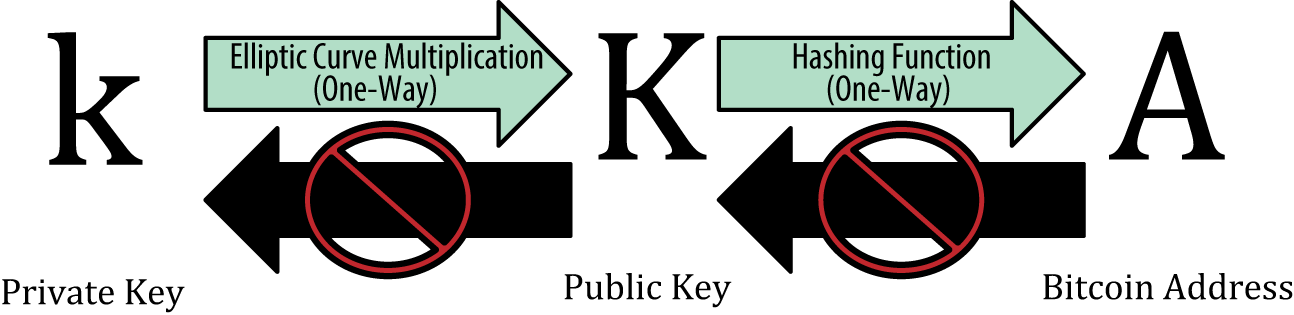
\includegraphics[width=\textwidth]{images/public_and_private_key.png}
	\caption{Generierung der Schlüssel bzw. Adressen aus dem jeweiligen Vorgänger}
	\label{6braun:fig:keys}
\end{figure}
\subsubsection{Private Keys}
Ein privater Schlüssel besteht aus einer Zahl von 256 zufälligen Bits. Er wird zum Signieren von Transaktionen und für den Zugriff auf ein Guthaben benötigt. Ohne privaten Schlüssel verliert man als Besitzer von Bitcoin auch den Zugriff auf das eigene Guthaben.\\
Um einen privaten Schlüssel generieren zu können, benötigt man eine sichere Quelle für "Zufälligkeit". In anderen Worten: Die Wahl der zufälligen Zahl darf nicht vorhersehbar sein. Dazu verwendet die Bitcoin-Software den Random Number Generator des verwendeten Betriebssystems kombiniert mit einem menschlichen Input, wie dem Bewegen der Maus. Mithilfe des Generators erzeugt man einen zufälligen String, welcher \emph{mehr} als 256 Bits hat. Diesen lässt man anschließend durch den SHA256 Hash-Algorithmus laufen und prüft, ob die resultierende Zahl kleiner ist, als die vom Bitcoin-Protokol gewählte Konstante \emph{n} ($n = 1.1578 * 10^{77}$).

\subsubsection{Public Keys}
Um einen öffentlichen Schlüssel aus dem Privaten generieren zu können, benötigt man ein kryptografisches Verfahren, welches eine Rekonstruktion des Privaten aus dem öffentlichen Schlüssel nicht zulässt.
Das vom Bitcoin-Protokol verwendete Verfahren wird \emph{Elliptic Curve Cryptography} gennant und bedient sich an den Eigenschaften einer Ellipse.
\begin{figure}[htpb]
	\centering
	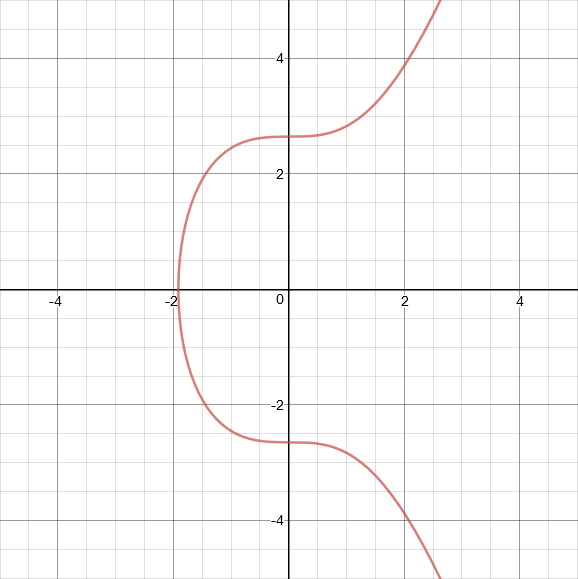
\includegraphics[width=0.7\textwidth]{images/elliptic_graph_cryptography.png}
	\caption{Die von Bitcoin verwendete Ellipse mit der Funktion $y^{2} = x^{3} + 7$ \\TODO: Bessere Grafik}
	\label{6braun:fig:ellipse}
\end{figure}
Um einen öffentlichen Schlüssel zu generieren, wählt man einen Punkt, den sogenannten Generatorpunkt, auf der Ellipse und Multipliziert diesen mit dem vorher generierten privaten Schlüssel. Eine Multiplikation kann auch als Addition einer Zahl mit derselben betrachtet werden. Um den Punkt G auf der Ellipse mit sich selbst zu addieren, zieht man an diesem die Tangente und berechnet den Schnittpunkt von Ellipse und der gezogenen Tangente. Anschließend spiegelt man den Punkt an der x-Achse, erhält 2G. Diese Addition führt man so oft aus, wie der 256 Bit lange private Schlüssel groß ist, sodass man am Ende einen Punkt (x,y) erhält, welcher als öffentlicher Schlüssel genutzt werden kann. Diesen generierten Schlüssel kann man veröffentlichen, denn aus ihm lässt sich nicht schließen, mit welchem Faktor der Generatorpunkt multipliziert wurde.

\subsubsection{Bitcoin Adressen}
Eine Adresse ist ein aus dem öffentlichen Schlüssel generierter String aus Buchstaben und Zahlen, der den Besitzer des Schlüssels zu einem potentiellen Empfänger einer Transaktion macht. Beim diesem muss es sich allerdings nicht zwangsläufig um eine Person handeln, denn auch Organisationen, geschriebene Skripte, etc. kommen als \emph{abstrakter} Empfänger in Frage.\\
So wie der Öffentliche aus dem privaten Schlüssel erzeugt wird, wird die Bitcoin Adresse aus dem öffentlichen Schlüssel mithilfe von Hashing-Algorithmen erzeugt. 
Die verwendeten Algorithmen, welche nacheinander auf den öffentlichen Schlüssel angewendet werden, heißen SHA-256 und RIPEMD160.\\
Da Verschlüsselungsalgorithmen einen Grundbaustein für Blockchain-Technologie darstellen, wird ihre Funktionsweise im Folgenden beispielhaft anhand des SHA-256-Algorithmus erläutert. 

\subsection{Einschub: SHA-256}
Ein Hashalgorithmus ist eine mathematische Funktion, die einen Input entgegennimmt und einen Output fester Größe, den sogenannten Hashwert erzeugt. Ein Algorithmus sollte idealerweise folgende Eigenschaften bieten:
\begin{itemize}
	\item Für einen gegebenen Input immer denselben Output generieren
	\item Nur in eine Richtung berechenbar sein
	\item Durch geringe Änderungen am Input einen völlig anderen Output generieren
\end{itemize}

Hashfunktionen haben vielerlei Anwendungsmöglichkeiten im Bereich der Datensicherheit und eine verwendete Hashfunktion im Bitcoin-Protokoll ist die bereits erwähnte SHA256-Funktion, welche u.A. von der NSA entwickelt wurde. Das folgende Unterkapitel orientiert sich an \cite{dang_2015}, ist allerdings für das Verständnis nachfolgender Kapitel nicht zwingend erforderlich.\\

\subsubsection{Definitionen}
Bevor der Algorithmus erläutert werden kann, ist es notwendig folgende Operationen, sowie benötigte Konstanten zu definieren. Die Operationen werden auf Zahlen in Binärform bitweise angewendet.
\begin{longtable}{p{3.5cm}p{10.5cm}l}
\caption{Benötigte Operationen}
	
		\\\toprule
		+  & Addition in Mod 2$^{32}$
		\\\midrule
		XOR  & Vergleichender Operator $\oplus$. Ergebnis ist True(1), wenn genau einer der beiden Inputs True ist. Andernfalls wird False(0) ausgegeben. Beispiel: $$0 \oplus 1 = 1$$
		\\\midrule
		Rotation Right  & Verschiebung der Bits um n Stellen nach rechts. Bei Overflow werden Bits wieder vorne angefügt. Beispiel: $$ROTR_1(011) = 101$$
		\\\midrule
		Shift Right  & Ähnlich wie die Rotation, nur dass Bits an letzter Stelle wegfallen und eine Nullen vorne angefügt werden. Beispiel: $$SHR_1(011) = 001$$
		\\\midrule
		Choice  & Nimmt drei Zahlen gleicher Länge entgegen und entscheidet anhand der Bits des ersten Parameters, welches Bit der jeweils anderen Parameter übernommen werden soll. $$Ch(x,y,z) = (x \land y)\oplus(\lnot x \land z)$$
		Beispiel: $Ch(110,001,101) = 001$
		\\\midrule
		Majority  & Nimmt drei Zahlen gleicher Länge entgegen und übernimmt an jedem Bit denjenigen Wert, der zwischen den Inputs am häufigsten auftaucht.
		$$Maj(x,y,z) = (x \land y)\oplus(x \land z)\oplus(y \land z)$$
		Beispiel $Maj(110,001,101) = 101$
		\\\midrule
		$\sigma_0$  & $\sigma_0$ und die folgenden Funktionen sind definierte Folgen der oben definierten Operationen.
		$$\sigma_0(x) = ROTR_7(x) \oplus ROTR_{18}(x) \oplus SHR_3(x)$$ 
		\\\midrule
		$\sigma_1$  & $$\sigma_1(x) = ROTR_{17}(x) \oplus ROTR_{19}(x) \oplus SHR_10(x)$$
		\\\midrule
		$\Sigma_0$  & $$\Sigma_0(x) = ROTR_2(x) \oplus ROTR_{13}(x) \oplus ROTR_{22}(x)$$
		\\\midrule
		$\Sigma_1$  & $$\Sigma_1(x) = ROTR_6(x) \oplus ROTR_{11}(x) \oplus ROTR_{25}(x)$$
		\\\bottomrule
\end{longtable}
Außerdem müssen noch zwei Listen mit Konstanten definiert werden. Die Liste K beinhaltet die ersten 32 Bit der Nachkommastellen der Kubikwurzeln der ersten 64 Primzahlen.
H die ersten 32 Bit der Nachkommastellen der Quadratwurzeln der ersten 8 Primzahlen. 
 Die genauen Werte haben keine sonderliche Bedeutung, sondern lediglich die scheinbare Zufälligkeit ist von Relevanz. Indem man diese berechenbaren Zahlen nimmt, minimiert sich die Wahrscheinlichkeit für eine mögliche Backdoor im Algorithmus.
\begin{lstlisting}[caption={Liste K von Konstanten},captionpos=b]
	428a2f98 71374491 b5c0fbcf e9b5dba5 3956c25b 59f111f1 923f82a4 
	ab1c5ed5 d807aa98 12835b01 243185be 550c7dc3 72be5d74 80deb1fe 
	9bdc06a7 c19bf174 e49b69c1 efbe4786 0fc19dc6 240ca1cc 2de92c6f 
	4a7484aa 5cb0a9dc 76f988da 983e5152 a831c66d b00327c8 bf597fc7
	c6e00bf3 d5a79147 06ca6351 14292967 27b70a85 2e1b2138 4d2c6dfc
	53380d13 650a7354 766a0abb 81c2c92e 92722c85 a2bfe8a1 a81a664b 
	c24b8b70 c76c51a3 d192e819 d6990624 f40e3585 106aa070 19a4c116 
	1e376c08 2748774c 34b0bcb5 391c0cb3 4ed8aa4a 5b9cca4f 682e6ff3 
	748f82ee 78a5636f 84c87814 8cc70208 90befffa a4506ceb bef9a3f7 
	c67178f2
\end{lstlisting}
\begin{lstlisting}[caption={Liste H mit den Arbeitsvariablen H0 - H7},captionpos=b]
	H0 = 6a09e667
	H1 = bb67ae85
	H2 = 3c6ef372
	H3 = a54ff53a
	H4 = 510e527f
	H5 = 9b05688c
	H6 = 1f83d9ab
	H7 = 5be0cd19
\end{lstlisting}
Die Zahlen befinden sich zu diesem Zeitpunkt in Hexadezimal-Form, müssen aber in Binärzahlen umgewandelt werden.
\subsubsection{Vorbereitung der Nachricht}
Bevor eine Nachricht verarbeitet werden kann, muss sie in eine für den Algorithmus brauchbare Form gebracht werden. 
Da der SHA-256 mit Zahlen in Binärform arbeitet, müssen Inputs in Stringformat über die ASCII-Tabelle in Binärzahlen umgewandelt werden. So wird z.B. aus dem String 'ab' die Zahl 01100001 01100010.
Anschließend fügt man eine Eins und k-viele Nullen hinzu, dass ein Vielfaches von 512 abgezogen 64 herauskommt. \cite{dang_2015} definiert diese Voraussetzung durch
$$l+1+k \equiv 448 Mod512$$
mit l als Länge der Nachricht. Anschließend werden 64 Bits hinzugefügt, welche die Zahl l repräsentieren, im Fall 'ab' wäre das die 16 in 64-Bit Repräsentation. Die resultierende N*512-Bit Zahl stellt den Input für die eigentliche Verschlüsselung dar.

\subsubsection{Aufteilung der Nachricht in Blöcke}
Die resultierende Zahl wird anschließend in Nachrichtenblöcke $M_1$ - $M_N$ der Länge 512-Bit und diese wiederum in 16 32-Bit-Blöcke $M_{i0}$ - $M_{i15}$ aufgeteilt, die man auch Wörter nennt. Der String 'ab' resultiert in einer 512-Bit-Zahl, sodass an dieser Stelle nur eine Aufteilung in 16 32-Bit-Blöcke nötig wäre.

\subsubsection{Algorithmus}
Im folgenden soll der Algorithmus anhand eines Pseudo-Codes erläutert werden. Zu beachten ist, dass die Liste k, sowie die Variablen H0-H7 global definiert seien.
\begin{lstlisting}[mathescape]
	For i=1 to N:
		w = []
		For t=0 to 63:
			if t <= 15:
				w.push(M[i][t])
			else:
				a = $\sigma_1$(w[t-2]) + w[t-7] + $\sigma_0$(w[t-15]) + w[t-16]
				w.push(a)
		a = H0
		b = H1
		c = H2
		...
		h = H7
		For j=0 to 63
			T1 = h + $\Sigma_1$(e) + Ch(e,f,g) + k[j] + w[j]
			T2 = $\Sigma_0$(a) + Maj(a,b,c)
			h = g
			g = f
			e = d + T1
			d = c
			c = b
			b = a
			a = T1 + T2
		H0 = a + H0
		H1 = b + H1
		...
		H7 = h + H7
	result = ''.concat(H1).concat(H2). ... .concat(H7)
\end{lstlisting}
Es wird zu Beginn ein leerer String initialisiert, der am Ende das Ergebnis des Algorithmus darstellt [1].\\
Anschließend wird die erste Schleife gestartet, die für jeden der N 512-Bit-Blöcke durchlaufen wird. Zu Beginn jedes Schleifendurchlaufs wird eine leere Liste \emph{w} initialisiert, die während des Durchlaufs gefüllt wird [2-3].\\
Für das Füllen der Liste wird eine weitere Schleife initialisiert, die von 0 bis 63 läuft und in den ersten 16 Durchgängen lediglich die 16 Wörter aus M[i] in die bisher leere Liste w einfügt [4-6]. \\
Ab Schleifendurchgang 16 werden die übrigen Einträge mithilfe der vorher definierten Funktionen berechnet, sodass man am Ende eine Liste mit 64 Einträgen hat [7-9].\\
Anschließend werden die sogenannten Arbeitsvariablen a bis h mithilfe der vorher definierten H0-H7 initialisiert [10-14].\\
Die folgende Schleife ist die, in der die eigentliche Kompression stattfindet. Sie läuft erneut von 0 bis 63 [15].\\
Mithilfe der vorher Definierten Funktionen und der Arbeitsvariablen werden die temporären Variablen T1 und T2 ermittelt. 
Für T1 spielen zusätzlich die Listen k, welche die Kubikzahlen der ersten 64 Primzahlen enthält, und die Liste w, welche die in Zeile 4 bis 9 generierten Wörter enthält, eine Rolle [16-17].\\
Anschließend werden die Arbeitsvariablen mithilfe der Temporären neu gesetzt, sodass man nach 64 Durchläufen scheinbar willkürliche Zahlen erhält [18-24].\\
Man addiert schließlich die Arbeitsvariablen und ursprünglichen Variablen H0-H7 und kettet diese aneinander. Bei einer kleinen Nachricht wie dem 'ab', welche lediglich einen 512-Bit-Block benötigt, wäre dies bereits das Ergebnis des Algorithmus. Sollte der Input ein Vielfaches von 512-Bit benötigen, wird die äußerste Schleife mehrfach durchlaufen und die Variablen H0-H7 in den Zeilen 25-28 nicht mehr mithilfe der initial definierten H0-H7, sondern mit denen der vorangegangenen Iteration berechnet.\\
Unabhängig von der Länge des Inputs erhält man so immer einen Output von 256 Bits, da die Arbeitsvariablen jeweils eine Länge von 32 Bits haben.

\subsection{Wallet}
Eine Wallet ist ein Programm, welches als Interface zwischen Bitcoin-Netzwerk und dem Nutzer dient. 
Dessen Funktionen beinhalten die Verwaltung der Schlüssel, das Berechnen des Guthabens und das Signieren von Transaktionen.
Eine Wallet ist, im Gegensatz zu einer physikalischen Geldbörse nicht für das Halten von Münzen, sondern zur Verwaltung der privaten Schlüssel zuständig. 
Wie das Berechnen des "Guthabens" geschieht, wird im Unterkapitel \emph{Transaktionen erläutert}.\\
Man unterscheidet zwischen nicht-deterministischen und deterministischen Wallets. Die erste Variante kann man sich als Korb vorstellen, in dem vorher zufällig generierte private Schlüssel in großer Anzahl gelagert sind. Dabei erzeugt ein Privater einen öffentlichen Schlüssel, der wiederum eine Adresse erzeugt (siehe Kapitel \emph{Keys und Adressen}).
Um die eigene Pseudonymität zu schützen ist es empfehlenswert, einen Key nur ein Mal zu benutzen. Aufgrund der hohen Anzahl angesammelter Keys und der damit verbundenen Datensicherung ist diese Art Wallet heute nicht mehr der Standard.\\
\begin{figure}[htpb]
	\centering
	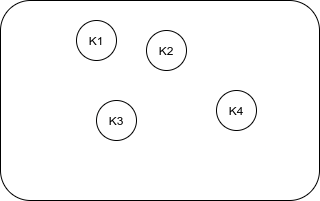
\includegraphics[width=0.7\textwidth]{images/non_det_wallet.png}
	\caption{Nicht-deterministische Wallet}
	\label{6braun:fig:non-deterministic_wallet}
\end{figure}
Die fortgeschrittenste Form einer Deterministischen ist die sogenannte BIP32-Wallet, welche 2 nützliche Eigenschaften aufweisen kann (BIP steht für \emph{Bitcoin Improvement Proposal} und bezeichnet eine nachträgliche Ergänzung zum Bitcoin-Ökosystem).\\
Diese werden in \cite{buterin_2013} als \emph{Master Public Key Property} und \emph{Hierarchy Property} bezeichnet.
Die Master Public Key Property beschreibt die Möglichkeit, aus einem Master Private einen Master Public Key zu generieren, der wiederum alle öffentlichen Schlüssel und deren Adressen erzeugen kann. Dazu berechnet man den sogenannten Offsets, indem man den gewünschten Index und den Master Public Key addiert und das Ergebnis als Input für eine Hashfunktion verwendet. Anschließend addiert man Offset und Master Public Key und erhält den öffentlichen Schlüssel am Index.
$$offset = SHA256(index + masterPubKey)$$
$$pubKey_{index} = offset + masterPubKey$$ Dies geht analog genauso mit dem Master Private Key. 
Aufgrund dieser Eigenschaft ist es möglich, den Master Public Key ungeschützt zu lagern und sogar an dritte Parteien herauszugeben, ohne dass diese Zugriff auf das Guthaben erhalten.\\
Die Hierarchieeigenschaft wird im Kontext einer Organisation mit verschiedenen Organisationszweigen interessant. Ein Geschäftsführer könnte so den unterschiedlichen Geschäftszweigen seines Unternehmens Schlüsselpaare zuweisen, wodurch diese die Verfügungsgewalt über das Eigene und Guthaben von Unterstellen erhalten. Gleichzeitig behält der Geschäftsführer die absolute Kontrolle über alle Schlüssel, da er im Besitz der Master Keys ist. 
\begin{figure}[htpb]
	\centering
	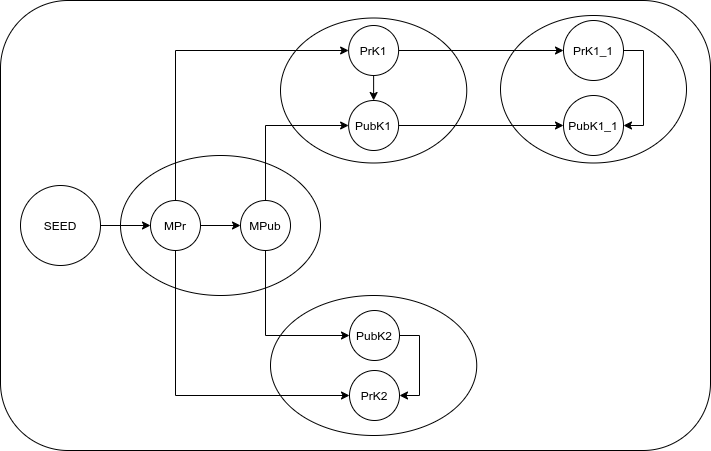
\includegraphics[width=0.7\textwidth]{images/bip32_wallet.png}
	\caption{BIP32-Wallet}
	\label{6braun:fig:non-deterministic_wallet}
\end{figure}
Anders als bei einer nicht-deterministischen Wallet müssen nicht mehr die Private Keys selbst, sondern lediglich der \emph{Seed} gesichert werden. Dieser ist seit dem BIP39/44 eine kurze Liste von für den Menschen leserlichen Worten. Diese können mithilfe eines speziellen Dictionaries in Hex-Zahlen umgewandelt werden, aus denen schließlich der Master Private Key erzeugt wird.
\subsection{Transaktionen}
Damit Bitcoin die Funktion des Zahlungs- bzw. Tauschmittels erfüllen kann, müssen Transaktionen vom Netzwerk ermöglicht werden. In einem \emph{Distributed Ledger}, einer Art dezentraler Datenbank, werden alle Transaktionen im Netzwerk aufgezeichnet. Da es sich um ein gänzlich digitales und dezentrales Netzwerk handelt, sind spezielle Datenstrukturen und Mechanismen nötig.\\
\subsubsection{Transaction Outputs}
Das Guthaben einer Wallet befindet sich nicht an einem Ort, sondern wird aus \emph{Unspent Transaction Outputs}, kurz UTXO zusammengesetzt, welche alle verfügbaren Gutschriften aus vergangenen Transaktionen darstellen.
Eine Wallet scannt die Blockchain nach allen Outputs, welche mit den Keys des Besitzers assoziiert sind und errechnet damit das gesamte verfügbare Guthaben. Außerdem speichert sie die nötigen Referenzen für den Zugriff auf die UTXO für den späteren Gebrauch in einer Datenbank ab.\\
UTXO¸ sind diskrete, sowie unteilbare Einheiten und können demnach nur in ihrer Gesamtheit genutzt werden. Man betrachte die folgende Abbildungen:
\begin{figure}[htpb]
	\centering
	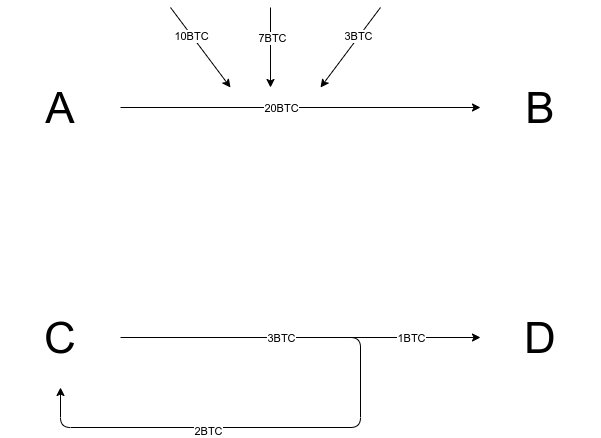
\includegraphics[width=0.7\textwidth]{images/UTXO.png}
	\caption{Transaktionen mit unteilbaren UTXO}
	\label{6braun:fig:Transaktionen}
\end{figure}
Für die gewünschte Transaktion von A nach B werden 20 BTC benötigt, die von der Wallet aus verfügbaren UTXO zusammengefügt werden. 
Für das optimale Zusammensammeln von Outputs ist die Wallet zuständig.\\
C hat für die gewünschte Transaktion von 1 BTC nur 3 BTC zur Verfügung, weshalb diese in ihrer Gesamtheit aufgebraucht werden müssen.
Die übrigen 2 BTC gehen jedoch nicht verloren, sondern landen lediglich wieder als Wechselgeld bei C. 
Die gewünschte Transaktion hat also 2 Outputs.\\
Jeder Output besteht aus 2 Komponenten: Der Anzahl von BTC und einem sogenannten \emph{Locking Script}, welches nur mithilfe des assoziierten private Keys gelöst werden kann. 
\subsubsection{Transaction Inputs}
Das Gegenstück zu den Outputs sind Inputs, über welche die benötigten UTXO für eine Transaktion gesammelt werden. Sie bestehen aus:
\begin{itemize}
	\item Einer ID, über die eine bestimmte Transaktion referenziert wird
	\item Vout, einem Index über den auf bestimmte UTXO der zuvor referenzierten Transaktion zugegriffen wird
	\item Dem Unlocking Script, welches das Locking Script des ausgewählten UTXO löst und mithilfe des privaten Schlüssels erzeugt wird
	\item Einer Sequence, einem optionalen Feld zur Sperrung der Outputs für eine bestimmte Zeit
\end{itemize}
Sowohl Input, als auch Output werden serialisiert und als Byte-Streams im Netzwerk propagiert.\\
\subsubsection{Transaktionskosten}
Abhängig von der Auslastung des Netzwerkes wird eine dadurch bestimmte Menge an Transaktionsgebühren nötig, die sowohl als Anreiz für Bitcoin-Miner, als auch Abschreckungsmechanismus gegen Angriffe durch hochfrequentes Senden von kleinen Transaktionen dienen.\\
Diese sind zwar kein Muss, jedoch bevorzugen die Miner Transaktionen mit höheren Transaktionskosten. 
Das berechnen von optimalen Transaktionsgebühren wird normalerweise von der Wallet ausgeführt, jedoch können auch manuelle Transaktionen erstellt werden, die ohne Transaktionskosten langsamer oder gar nicht vom Netzwerk verarbeitet werden.
Bei einer manuellen Transaktion müssen sowohl Inputs, als auch Outputs definiert werden und die Transaktionsgebühren ergeben sich implizit aus der Differenz jener Komponenten. So wie man keine Transaktionsgebühren angegeben kann, ist auch das versehentliche Angeben von zu hohen Gebühren möglich. Man betrachte erneut die Abbildung \ref{6braun:fig:Transaktionen}, in der C 3 BTC an D sendet. Die Transaktion hat 2 Outputs, 1 BTC an D und 2 BTC zurück an C. Sollte der Sender vergessen den 2. Output, welcher das Wechselgeld darstellt, zu definieren, dann werden die gesamten 2 BTC als Transaktionsgebühren für die Transaktion genutzt.\\

Zusammenfassend lassen sich Transaktionen als Sammlungen von Inputs und Outputs definieren, deren Differenz die genutzten Transaktionskosten darstellen.
 
\subsection{Die verschiedenen Akteure im Netzwerk}
\subsection{Der Konsensalgorithmus Proof-of-Work}
\subsection{Angriff auf das Netzwerk}


    \chapter{Blockchain 2.0}
Durch den Zusammenschluss verschiedenster Vorgängertechnologien gelang es Nakamoto, einen dezentralen Mechanismus zur Verarbeitung von Transaktionen vorzustellen, der mit den bereits bestehenden Institutionen in Punkten wie Sicherheit und Geschwindigkeit konkurrieren kann. Vor allem die Möglichkeit, auf eine dezentrale Art und Weise zu einem gemeinsamen Konsens kommen zu können, macht es zu einer disruptiven Technologie. Als Programmierer:innen jedoch Konzepte, die über das Versenden von Guthaben hinausgehen, entwickeln wollten, wurde dies durch die Einschränkungen des Bitcoin-Protokolls, wie die Block-Dauer von 10 Minuten oder unzureichende Block-Struktur, erschwert. Man kann deshalb von Bitcoin als spezialisierte Blockchain, die ihre wenigen Funktionalitäten zufriedenstellend bereitstellt, reden.\\

Im Jahr 2013 veröffentlichte \cite{buterin_whitepaper_2013} ein Whitepaper, in dem er Konzepte für eine neue Blockchain namens Ethereum vorstellte. Dabei handelt es sich um den Entwurf für eine Art Welt-Computer, der sich von Bitcoin vor Allem in den folgenden Punkten unterscheidet:
\begin{enumerate}
	\item Es können beliebige Daten auf der Blockchain gespeichert werden
	\item Es kann Code auf der Blockchain hinterlegt und dort ausgeführt werden
	\end{enumerate}
Im Gegensatz zum Bitcoin-Protokoll, welches zwischen den Blöcken nur eine Veränderung des UTXO-Sets aufweist, stellt Ethereum einen globalen State dar, in dem neben den Aufzeichnungen zu den Guthaben der Teilnehmer:innen auch andere beliebige Daten abgespeichert werden können. Damit geht Ethereum über den Einsatz als Geldsystem hinaus.
Über spezielle Adressen erlaubt das Ethereum-Protokoll das Hinterlegen von kompiliertem Code direkt auf der Blockchain, welcher über Transaktionen getriggert werden und den State modifizieren kann. 
\\

Ethereum übernimmt viele Konzepte, die bereits aus dem Kapitel \emph{Blockchain 1.0} bekannt sind (Keys, Wallets, Mining, etc.). Dieses Kapitel befasst sich mit Neuerungen, die das Ausführen von Smart Contracts ermöglichen bzw. durch diese ermöglicht werden. Außerdem werden mögliche Use-Cases, welche durch die Neuerungen ermöglicht werden, beschrieben. Dieses Kapitel orientiert sich an \cite{antanopoulos_2018} und zitiert, wo es nötig ist, zusätzlich.
\section{Neuerungen unter Ethereum}
Im Gegensatz zum Bitcoin-Protokoll, in dem das UTXO-Modell genutzt wird, kommt beim Ethereum-Protokoll ein sogenanntes \emph{Account Based Model} zum Einsatz, welches im Bereich Datenschutz dem UTXO-Modell aus Bitcoin unterlegen sein soll \cite[]{beres_2020}. Jede Adresse auf der Blockchain hat ein Guthaben, auf das Ether, die native Währung auf Ethereum, hinzugefügt bzw. abgehoben werden kann. Eine passende Analogie für die beiden Kontenmodelle wäre das UTXO-Modell als physikalische Geldbörse, aus der für eine Transaktion einzelne Münzen (UTXO) herausgesucht und konsumiert werden müssen, sowie das Girokonto, dessen Guthaben beliebig augmentiert werden kann. Dies hat zur Folge, dass es andere Mechanismen zum Lösen des Double-Spending-Problems geben muss.

\subsection{Transaktionen}
Neben dem Transfer von Guthaben, so wie es bereits von Bitcoin bekannt ist, dienen Transaktionen auf Ethereum dem Zweck, die Ausführung von, auf der Blockchain hinterlegten, Smart Contracts auszulösen.
Um diese Funktion erfüllen zu können, unterscheidet sich laut \cite{antanopoulos_2018} eine Transaktion auf Ethereum zu deren im Bitcoin-Protokoll:
\begin{lstlisting}[caption={Struktur einer Transaktion in Ethereum.},captionpos=b]
	Transaction {
		nonce;
		recipient;
		value;
		data;
		v;
		r;
		s;	
		gas_price;
		gas_limit;
}
\end{lstlisting}
\emph{Nonce} ist ein Zähler, der bei Transaktionen auf Ethereum eine andere Bedeutung hat, als beim Mining. In einer Transaktion gibt er an, wie viele bestätigte Transaktionen, inklusive sich selbst, bereits von jener Adresse gesendet wurden. Dies führt dazu, dass das Netzwerk eine Warteschlange, aus den von einer Adresse gesendeten Transaktionen, bilden kann. Da im Account-Based-Modell keine UTXO konsumiert werden, kann das Netzwerk anhand des Zählers eine Priorisierung der unbestätigten Transaktionen festlegen und, sollte das gesamte Guthaben nicht ausreichen, Transaktionen mit niedrigerer Priorität ablehnen.
Der eigentliche Payload einer Transaktion besteht aus \emph{Value} und \emph{Data}, wobei keines dieser Felder zwingend gefüllt sein muss.
Als Value bezeichnet man die Ether, welche bei einer Transaktion gesendet werden können und je nach Art der Empfängeradresse anders verarbeitet werden. Findet die Transaktion zwischen zwei Teilnehmer:innen des Netzwerkes statt, so werden die Ether der Empfängeradresse zugeschrieben. Handelt es sich dagegen um einen Smart Contract, so wird dessen Guthaben (ein Smart Contract hat eine Adresse und kann dementsprechend Ether halten) erhöht und eine, als \emph{payable} gekennzeichnete, Fallback-Funktion ausgeführt. Bei Fehlen einer solchen Funktion wird ein Fehler geworfen und andernfalls der State des Smart Contracts angepasst.
Die Fallback-Funktion wird nur dann ausgeführt, wenn das Feld Data des Payloads leer ist. In diesem selektiert man die gewünschten Funktionen und mit welchen Parametern diese ausgeführt werden sollen. Die Felder \emph{v, r ,s} sind für die Authentifizierung nötig, werden hier aber nicht weiter erörtert. Im Endeffekt werden Transaktionen wie bekannt mit dem privaten Schlüssel signiert und andere Teilnehmer:innen des Netzwerkes validieren diese mit dem öffentlichen Schlüssel.\\
\subsection{Neues Konzept: Gas}
In seinem Paper \cite{turing_1936} stellte Alan Turing einen Entwurf für eine Maschine vor, die aus einem nahezu unendlich langem Streifen aus Papier und einem Kopf besteht. Der Streifen ist in Bereiche unterteilt, die jeweils ein Zeichen, wie z.B. eine Zahl, enthalten und zwischen denen sich der Kopf bewegen kann. Dieser ist in der Lage, das Zeichen des Bereiches, auf dem er sich befindet, zu lesen, zu überschreiben, zu löschen oder auch auf dem Streifen zu verschieben. Die Maschine ermöglicht somit, in Abhängigkeit zu den gegebenen Instruktionen, das Berechnen sowie abspeichern beliebiger Sequenzen von Zeichen auf dem Streifen. Eine solche Maschine wird heutzutage als Turing-Maschine bezeichnet.\\

Im Ethereum-Whitepaper \cite{buterin_whitepaper_2013} wird Ethereum als Blockchain bezeichnet, die eine Programmiersprache verwendet, welche turing-vollständig ist. \cite{Michaelson_2020} beschreibt turing-vollständige Programmiersprachen als solche, die ihre Berechnungen in Form einer Turing-Maschine ausdrücken können. Dafür dürfen sie laut Michaelson weder in ihren genutzten Werten, noch in den darauf ausgeführten Berechnungen beschränkt sein. Konkret heißt das im Fall von Ethereum und der genutzten Programmiersprache, dass beliebig aufwendige Berechnungen, sowie geforderter Speicherbedarf ermöglicht werden müssen.
Auf einem lokalen Computer kann eine endlos laufende Schleife leicht gestoppt werden, aber im Kontext eines dezentralen Systems würde jene Schleife die Stabilität des gesamten Netzwerkes bedrohen und würde sogar als Angriffsmethode für bösartige Akteur:innen dienen können. Im Endeffekt nutzen die Teilnehmer:innen des Netzwerkes Ressourcen aus demselben Pool, sodass ein Mechanismus nötig ist, um das Verschwenden dieser begrenzten Ressourcen unattraktiv zu machen.\\

Die Anweisungen, welche in einem Smart Contract hinterlegt sind, werden nach Triggern durch eine Transaktion von der \emph{Ethereum Virtual Machine} interpretiert und ausgeführt. Jede der Anweisungen verbraucht jedoch \emph{Gas}, welches als neues Konzept zur Lösung der genannten Probleme aus Turing-Vollständigkeit eingeführt wurde. So bleibt die Programmiersprache zwar turing-vollständig, die Ressourcen, welche Teilnehmer:innen in Anspruch nehmen können, werden jedoch begrenzt. Dies hat zur Folge, dass die Anzahl an Gas, sowie der Preis in Ether, welchen man bereit ist zu zahlen, in einer Transaktion angegeben werden muss. Miner suchen sich anschließend die Transaktionen heraus, welche für sie attraktiv sind, und fügen sie zu ihrem Block hinzu. Übrig gebliebenes Gas wird in Form von Ether wieder zurückerstattet. Zu einer Transaktion gehören demnach die, für den Versand bestimmten, Ether, sowie jene, welche für den Erwerb von Gas bereitgestellt werden müssen.\newpage
\subsection{Ethereum Virtual Machine}
Genau wie im Bitcoin-Protokoll sammeln Miner Transaktionen, validieren diese und versuchen, per Proof-Of-Work einen geeigneten Block zu finden.
Im Gegensatz zu den Transaktionen im Bitcoin-Protokoll lösen die Transaktionen unter Ethereum allerdings die Ausführung von, auf der Blockchain hinterlegten, Smart Contracts aus. 
Für die Ausführung derer ist die Ethereum Virtual Machine (kurz EVM) zuständig. 
Sie ist eine Virtuelle Maschine, die in  \cite{wood_yellowpaper_2014} als stack-basierte Architektur beschrieben wird. 
Die folgende Abbildung 3.1 illustriert eine vereinfachte Darstellung ihrer Funktionsweise: 
\begin{figure}[htpb]
	\centering
	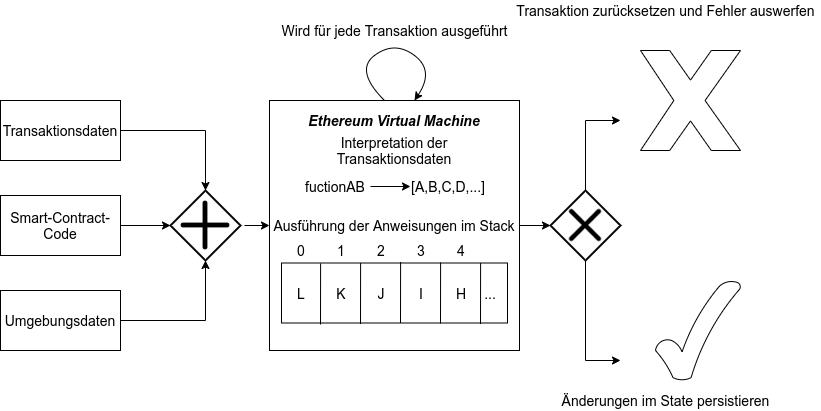
\includegraphics[width=\textwidth]{images/evm_simple.png}
	\caption{Vereinfachung der Ethereum Virtual Machine.\\
	Quelle: Eigene Darstellung}
	\label{6braun:fig:evm_simple}
\end{figure}\\
Die EVM erhält als externen Input die Daten für Transaktionen, die sie ausführen muss und wandelt die darin enthaltenen Funktionsaufrufe sowie ihre Parameter in ausführbare Einzeloperationen in Form von Maschinencode um. 
Als zusätzliche Inputs für die Verarbeitung von Transaktionen dienen sowohl der Smart-Contract-Code, als auch Umgebungsdaten, wie z.B. die verfügbare Menge an Gas oder das Guthaben der involvierten Adressen. 
Die EVM führt die Anweisungen nach dem LIFO-Prinzip im Kontext der Umgebungsdaten aus und verbraucht für jede Anweisung eine gewisse Menge Gas, die von der Art jener Operation abhängt. Wenn während der Ausführung keine Fehler auftreten, dann wird der State persistiert und mit der nächsten Transaktion fortgefahren. 
Wenn allerdings an einer beliebigen Stelle des Stacks ein Fehler auftritt, sei es beispielsweise durch unzureichendes Gas, wird die gesamte Transaktion zurückgesetzt, da Transaktionen atomar sind und nur in ihrer Gesamtheit ausgeführt werden können. Erst wenn ein valider neuer State erreicht ist, gilt der Block selbst als valide und kann mittels Proof-Of-Work gemined werden. Im Anhang unter \ref{6braun:fig:EVM_full} befindet sich eine umfassende Abbildung aus dem Buch \cite{antanopoulos_2018}.
\subsection{Die Programmiersprache Solidity}
Der Programmcode, welcher von der EVM interpretiert wird, ist in der Programmiersprache \emph{Solidity}, welche an andere objektorientierte Programmiersprachen wie Java oder Javascript erinnert, geschrieben. Sie bietet bekannte Funktionalitäten wie Kontrollstrukturen, Vererbung, etc. an, wobei man aufgrund der Verwendung von Gas auf die Wirtschaftlichkeit des Codes achten muss. Anhand des folgenden Codes soll kurz die Syntax von Solidity dargestellt werden: 
\begin{lstlisting}[caption={Beispielcode für Solidity},captionpos=b]
	// SPDX-License-Identifier: MIT
	pragma solidity ^0.8.3;
	
	contract AdvertContract {
		address owner;
		struct Ad {
			uint counter;
			uint funds;
		}
		mapping(uint => Ad) public ads;
		
		constructor() {
			owner = msg.sender;
		}
	
		receive() external payable {}
		function getBalance() public view returns(uint){
			return address(this).balance;
		}
}
	\end{lstlisting}
Zunächst werden sowohl die Lizenz, als auch die Version des gewünschten Compilers definiert [Zeile 1-2]. Der Befehl \emph{Contract} lässt sich mit einer Klasse aus anderen Programmiersprachen vergleichen. 
Es können einfache Felder [5], eigene Datenstrukturen [6-9], als auch sogenannte \emph{mappings} definiert werden [10]. Mappings lassen sich mit Hash-Tabellen vergleichen und über die Notation \emph{(uint => Ad)} gibt man an, dass über einen \emph{uint}, welcher für unsigned Integer steht, als Schlüssel auf Objekte des Typs Ad zugegriffen werden kann. 
Der Contract verfügt über einen Konstruktor, der nur einmal während des Deployments aufgerufen wird. In diesem kann beispielsweise diejenige Adresse festgelegt werden, die als Eigentümer des Contracts gelten soll. 
Während des Deployments wird eine spezielle Transaktion, welche den kompilierten Code enthält, an die Adresse \emph{0x00...} gesendet und von den Minern als Aufforderung für das Hinterlegen des Codes auf der Blockchain interpretieren. 
Die globale Variable \emph{msg} ermöglicht den Zugriff innerhalb des Contracts auf Informationen der Transaktion, welche diesen triggert [12-14].
\emph{Receive} stellt eine Fallback-Funktion dar, welche das Verhalten des Contracts für den Fall definiert, dass eine Transaktion mit leerem Feld 'data' diesen aufruft, was einer schlichten Überweisung gleicht [16]. Der Decorator \emph{payable} ist dann nötig, wenn eine, an diese Funktion gerichtete, Transaktion zusätzliche Ether mitschickt, denn anderenfalls wird ein Fehler ausgeworfen. \emph{External} macht, ähnlich wie der Decorator public, die Funktion nach außen hin sichtbar, ist jedoch bei der Verwendung von Gas effizienter. Über den Befehl \emph{function} lassen sich eigene Funktionen definieren für die man gewünschte Parameter, Zugriffsmodifikator angeben muss. Für den Fall, dass die Funktion einen Wert zurückgibt, muss ein Rückgabewert und bei ausschließlich lesendem Zugriff der Befehl \emph{view} angegeben werden [17-19]. Dies sind nur einige der in \cite{solidity_2021} aufgeführten Funktionalitäten.
\subsection{Mögliche Use-Cases}
\subsubsection{DAO}
\cite{buterin_whitepaper_2013} bezeichnet \emph{Decentralized Autonomous Organizations} als dezentrale Organisationen, in denen Parteien mit einer Mehrheit von 67\% des Stimmrechts über die Zukunft der Organisation, welche in Smart Contracts definiert ist, entscheiden dürfen. Darin ist festgelegt, wer zur Organisation gehört und ob bestimmte Mitglieder von ihr bezahlt werden. Eine 67\% Mehrheit könnte neue Mitglieder aufnehmen, entlassen oder deren Bezahlung anpassen.
\subsubsection{Tokens}
Als Token bezeichnet \cite[S. 315]{antanopoulos_2018} die Abstraktion einer bestimmten Sache auf der Blockchain, die man besitzen kann. Dies können sowohl wieder Währungen zum Bezahlen innerhalb des Systems sein, als auch physikalische Besitztümer wie Gold oder Immobilien. Token, welche einzigartige physikalische, als auch digitale Gegenstände repräsentieren, werden \emph{Non-fungible Token} genannt und der Vorteil dieser Token ist, dass der Besitz nicht durch eine zentrale Partei wie z.B. einen Staat, sondern durch den Besitz des dazugehörigen Keys definiert wird.
\subsubsection{DApps}
Klassische (Web-)Applikation bestehen meist aus den Front-, Backend und Datenbank. Das Vorhaben hinter \emph{Decentralized Applications} ist eine Dezentralisierung von Anwendungen, indem man bestimmte Funktionalitäten über Smart Contracts oder andere dezentrale Mechanismen bereitstellt. Dies hat den Vorteil, dass man sowohl Transparenz schafft (die Blockchain ist öffentlich und kann von allen Akteur:innen eingelesen werden), als auch die Abhängigkeit von Parteien, welche für die Infrastruktur der Anwendung verantwortlich sind, minimiert.
    \chapter{Blockchain im Online Advertising}
Die bisherigen Kapitel dienen dem Zweck, Lesenden ein Verständnis über technische, als auch funktionelle Aspekte der Blockchain-Technologie zu vermitteln. Allerdings ist Informationstechnologie kein Selbstzweck, sondern wird zur Lösung von konkreten Problemen verwendet.
Im folgenden Kapitel soll diese, im Kontext des \emph{Online Advertisings}, in einen wirtschaftlichen Prozess sinnvoll eingebaut werden. 
Dafür werden zunächst die Themen Online Advertising und speziell Programmatic Advertising näher beschrieben und mögliche Verbesserungen mittels Blockchain-Technologie erörtert. 
Ausgehend davon wird die Architektur und ihre Komponenten für eine Webanwendung, in die ein Smart Contract eingebaut ist, vorgestellt. 
\section{Online Advertising}
Laut \cite{johnson_2021} ist das Internet heutzutage fester Bestandteil des Lebens von 4,66 Milliarden Menschen auf der Erde, die es regelmäßig verwenden. Ein solch hoher Traffic macht das Schalten von Werbung attraktiv, sodass im Jahr 2020 laut \cite{statista_online_advertisement_revenue_2021} ein Umsatz von 139,8 Milliarden US-Dollar in den USA erzielt werden konnte. Die verschieden Arten von Werbung werden unter dem Begriff \emph{Online Advertising} gesammelt.
Im Paper \cite{bundeskartellamt_2018} wird Online Advertising, welches auch als Digital Advertising bezeichnet werden kann, als jegliche Art Werbung, die über das Internet auf mobilen, sowie Desktopanwendungen vermittelt wird, bezeichnet. Darin werden auch die relevante Unterkategorien beschrieben: 
\begin{itemize}
	\item Search Advertising: Werbeanzeigen werden auf den Oberflächen von Suchmaschinen entweder als Anzeigen seitlich der Suchergebnisse oder als Bestandteil dieser angezeigt
	\item Mobile Advertising: Auf Mobilgeräte angepasste Anzeigen, die auch Bestandteile von Apps sein können
	\item Social Media Advertising:
	Nutzer:innen mit einer hohen Reichweite bauen Werbung in ihre Inhalte ein. Diese Nutzer:innen nennt man auch \emph{Influencer}
	\item Display Advertising: Inhaber:innen von Webseiten bieten verfügbaren Platz als Werbeflächen an
\end{itemize}
Mit der ersten online-geschalteten Werbeanzeige im Jahr 1994 ist das Display Advertising die älteste Form des Online Advertisings und soll im Folgenden näher thematisiert werden \cite[]{bundeskartellamt_2018}.
\subsection{Display Advertising heute}
Die einfachste Form des Display Advertisings wäre die Übereinkunft zwischen Inhaber:innen, welche Werbung auf ihren Webseiten schalten und werbenden Unternehmen, die pro Schaltung bezahlen. In der Praxis würde dies allerdings einen hohen Aufwand für beide Parteien bedeuten. Unternehmen müssten einen Vertrag darüber aufsetzen, welche Werbung wie oft geschaltet werden sollte und Inhaber:innen der Werbefläche müssten sich selbst um das Darstellen der Anzeigen, als auch Tracking diverser Metriken, wie z.B. Impressionen oder Klicks, kümmern.\\

Als Folge dessen entstand das sogenannte \emph{Programmatic Advertising}, welches durch Fortschritte in Bereichen wie Rechenleistung, Datenspeicherung, Internetgeschwindigkeit, etc. zum dominanten Verfahren wurde \cite[6]{busch}. Es ermöglicht eine auktionsbasierte Verteilung von Werbeschaltungen, die völlig automatisiert möglichst geeignete Anzeigen während des Ladens einer Webseite zuweist \cite[]{alaimo_2018}. Dies hat aber auch zur Folge, dass mehr Komponenten in die Logistik der Anzeigenschaltung involviert sind. Es entsteht die folgende Konstellation aus Abbildung 4.1, die in \cite{optimity_advisors_2019} näher erläutert wird:

\begin{figure}[htpb]
	\centering
	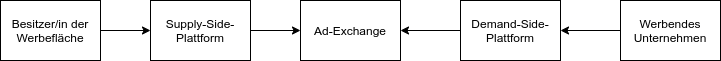
\includegraphics[width=\textwidth]{images/programmatic_advertising.png}
	\caption{Involvierte Parteien in gängigem Display Advertising.\\
	Quelle: vgl. \cite[S. 9]{optimity_advisors_2019}}
	\label{6braun:fig:programmatic_advertising}
\end{figure}
Die \emph{Supply-Side-Plattform} dient als Schnittstelle zwischen der Werbefläche und dem Auktionshaus, der \emph{Ad-Exchange}. Sie kümmert sich darum, dass eine Webseite mit Anzeigen versorgt wird, indem sich dessen Werbefläche beim Auktionshaus registriert. Außerdem analysiert sie eintreffende Besucher:innen und leitet gegebenenfalls Daten, die beispielsweise durch Nutzungsverhalten auf der Webseite oder Cookies gesammelt werden, an das Auktionshaus weiter. Auf der Unternehmensseite dient die \emph{Demand-Side-Plattform} als Schnittstelle zum Auktionshaus, welches den Unternehmen das zur Verfügung stellen von Anzeigen, sowie das Verfolgen von diversen Metriken ermöglicht. Im Auktionshaus kommt es schließlich zur Verteilung der Anzeigen in Echtzeit, indem verfügbare Werbeflächen und die Daten der Besucher:innen in diesem veröffentlicht werden. Die Demand-Side-Plattformen geben abhängig von den Daten Gebote ab und die Anzeige der gewinnenden Plattform wird schließlich der Webseite zum Anzeigen zur Verfügung gestellt.\\

In Deutschland entsprach der Anteil von Ausgaben für Programmatic Advertising im Jahr 2017 54\% und im Jahr 2018 70\% der gesamten Ausgaben für Online Advertising (eMarketer (2018) zitiert nach \cite[S. 21]{optimity_advisors_2019}). Der gesamte Markt für Online Advertising fällt mit 6,6 Milliarden Euro im Jahr 2017 laut \cite{optimity_advisors_2019} im Vergleich zum US-Markt jedoch gering aus.

Ein Beispiel für eine Supply-Side-Plattform ist \emph{AdSense} des Unternehmens \emph{Google}, welches Besitzer:innen mit einem Code-Snippet versorgt, die sie lediglich im Quellcode ihrer Webseite einfügen müssen. Über diese werden Anzeigen direkt auf die Seite geladen, ohne dass sie sich selbst darum kümmern müssen \cite[]{google_adsense_2021}. Zur Unternehmensseite hin fungiert \emph{Google Ads} desselben Unternehmens als Demand-Side-Plattform, über die Unternehmen Gebote für die, mittels Code-Snippet bereitgestellten, Anzeigeflächen abgeben. 
Zusätzlich dazu können Unternehmen diverse Metriken für erworbene Werbeflächen abrufen, die von Google Ads getrackt werden \cite[]{google_ads_2021}.\\

Auch wenn die Einbeziehung eines solchen Dienstleisters den vermittelten Parteien Aufwand erspart, entstehen dadurch nicht nur Vorteile.
Für Besitzer:innen von Werbeflächen entsteht der Nachteil, dass nicht das gesamte Geld von Unternehmen bei ihnen ankommt, weil in diesem Fall Google gleichzeitig den Zahlungskanal darstellt. 
Stattdessen erhalten diese 68\% des Umsatzes, wodurch in diesem Fall fast ein Drittel an das vermittelnde Unternehmen geht \cite[]{adsense_revenue_2021}. Auf Unternehmensseite entsteht der Nachteil fehlender Transparenz, denn Zugriff auf die getrackten Metriken erhält man nur über Vermittelnde. Außerdem besitzen die vertikal integrierten Unternehmen wie Google oder Facebook dadurch, dass sie alle Komponenten in der Dienstleistungskette abdecken, eine so hohe Marktmacht, dass laut \cite{cnbc_2017} im Jahr 2017 eine Marktdominanz von 73\%, sowie ein Anteil von 83\% am Gesamtwachstum der Industrie vorhergesagt wurde. Ein letzter wichtiger Punkt ist der fehlende Datenschutz im Programmatic Advertising. Die automatisierte Schaltung von relevanten Anzeigen ist nur deshalb möglich, weil personenbezogene Daten von Nutzer:innen erhoben werden, was eine Verletzung von Datenschutzrichtlinien zur Folge haben könnte \cite{palossanchez_2019}. Diese werden auch über Anwendungsgrenzen hinweg gesammelt und zur Verfügung gestellt, wie es beispielsweise bei Google und ihrem Tochterunternehmen \emph{Youtube} der Fall ist.

\subsection{Mögliche Verbesserungen mittels Blockchain-Technologie}
In \cite{campbell_2018} und \cite{paerssinen_2018} wird Blockchain-Technologie als mögliche Lösung für diese Probleme genannt, indem die Rahmenbedingungen für Interaktionen zwischen Besitzer:innen und Unternehmen mittels Smart Contracts geregelt werden. 
Da Ethereum das Hinterlegen beliebiger Daten ermöglicht, könnte in den Smart Contracts aufgezeichnet werden, wie oft eine Anzeige geschaltet wurde und welche Kosten dafür aufkommen. 
Aufgrund der Transparenz einer öffentlichen Blockchain können Unternehmen jederzeit auf darauf hinterlegte Metriken zugreifen. Gleichzeitig kann die Blockchain in ihrer ursprünglichen Funktion als direkter Zahlungskanal zwischen Besitzer:innen und Unternehmen genutzt werden. Als Folge dessen würden Vermittelnde als Intermediäre wegfallen und Vorteile für beide übrigen Parteien würden entstehen.
\section{Programmierung eines Proof-of-Concept}
Die Chancen, welche Blockchain-Technologie für das Display Advertising bieten könnte, sollen im Folgenden am Beispiel eines \emph{Proof-of-Concept} veranschaulicht werden. 
Dafür wird eine Webanwendung entwickelt, die beliebigen Inhalt abbildet und an den Seiten Platz zum Schalten von Anzeigen hat. 
Zusätzlich dazu sollen die soeben genannten Verbesserungen eingebaut werden, indem Unternehmen direkt auf der Seite eine Anzeige hochladen und eine Art Guthaben erwerben können, welches beim Schalten der Anzeige aufgebraucht wird. Die Unternehmen sollen in der Lage sein, die Anzahl der Schaltungen, als auch das übrige Guthaben abzurufen und bei Bedarf erhöhen zu können. Die Webanwendung soll den in Abbildung 4.2 illustrierten Aufbau haben:
\begin{figure}[htpb]
	\centering
	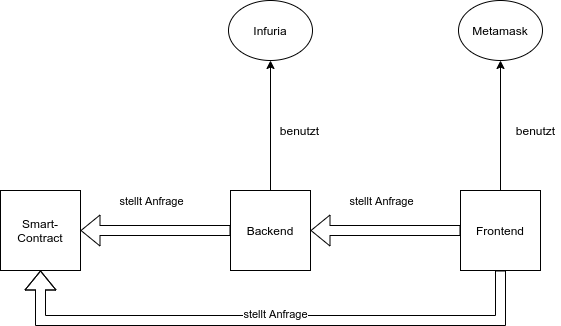
\includegraphics[width=\textwidth]{images/aufbau_PoC.png}
	\caption{Aufbau der Webanwendung.
	Quelle: Eigene Darstellung}
	\label{6braun:fig:aufbau_poc}
\end{figure}\\
Die Anwendung besteht aus einem Front- und Backend, sowie einem Smart Contract auf dem Ropsten-Testnetz \footnote{Es handelt sich um eine eigenständige Ethereum-Blockchain, auf der Entwickelnde ihre Smart Contracts, ohne den Verbrauch realer Ether, in einer vergleichbaren Umgebung testen können}. Sowohl Front-, als auch Backend können nicht direkt mit der Blockchain kommunizieren, sondern tun dies über sogenannte \emph{Provider}. In den folgenden Unterkapiteln sollen die einzelnen Komponenten näher erläutert werden.
\subsection{Frontend}
Das Frontend bildet den Teil der Anwendung, welcher im Browser von Nutzer:innen läuft. Es kümmert sich um die Visualisierung und Interaktionen mit den Nutzer:innen der Seite.
Für das Frontend wird das Framework \emph{Angular}, welches von Google in Stand gehalten wird, genutzt. Über einen einzigen Befehl \emph{ng new} auf der Kommandozeile lässt sich eine lauffähige Webanwendung generieren, die anschließend nach Belieben überarbeitet werden kann. Außerdem wird statt Javascript die Programmiersprache \emph{Typescript} genutzt, welche den Vorteil der Typsicherheit, wie sie beispielsweise aus Java bekannt ist, mitbringt. Ein letzter Vorteil unter vielen ist die Nutzung der Bibliothek \emph{RXJS}, welche eine Alternative zu bekannten Technologien wie Ajax zur Behandlung von asynchronen Funktionen bietet.
Zur Kommunikation mit der Blockchain wird die Bibliothek \emph{Ethers.js} genutzt. Sie erlaubt es Entwickler:innen, Anfragen an eine Blockchain-Node zu schicken, von der Transaktionen anschließend signiert und gesendet werden. Das Frontend lässt sich grob in die folgenden drei Elemente unterteilen:
\begin{itemize}
	\item Die Hauptkomponente, bestehend aus HTML-, CSS- und Typescriptdatei
	\item Der Api-Service, welcher sich um die Kommunikation mit dem Backend kümmert
	\item Der Blockchain-Service, welcher sich um die Kommunikation mit dem Smart Contract kümmert
\end{itemize}
Die Hauptkomponente existiert bereits nach der initialen Generierung und dient als Gerüst für die Anwendung. In Angular können Komponenten nach dem Bausteinprinzip beliebig angeordnet werden, sodass jede Komponente für einen anderen Teil der Anwendung zuständig sein kann. Auch eine hierarchische Anordnung ist möglich, sodass eine Komponente wieder andere enthalten kann. Sogenannte \emph{Services} können durch Deklaration im Konstruktor von Komponenten genutzt werden, dies nennt man \emph{Injecting}. Services sind keine eigenständigen Komponenten, sondern stellen lediglich Funktionalitäten bereit, wie z.B. die Kommunikation mit dem Backend. Einige wichtige Funktionen der Datei \emph{app.component.ts} sollen im Folgenden erläutert werden.
\subsubsection{Konstruktor und Laden von Bildern}
\begin{lstlisting}[caption={Konstruktor und Laden von Bildern im Frontend},captionpos=b]
public constructor(private sanitizer: DomSanitizer,
private api: ApiService,
private http: HttpClient,
private formBuilder: FormBuilder,
public blockService: BlockchainService) {
	this.getImageFromApi();
	this.getImageFromApi();
}

public getImageFromApi(): void {
	this.api.getImage().subscribe((baseImage: any) => {
		const blob = new Blob([baseImage]);
		const unsafeImg = URL.createObjectURL(blob);
		
		this.upperRight === undefined ?
		this.upperRight = this.sanitizer
						.bypassSecurityTrustUrl(unsafeImg) :
		this.upperLeft = this.sanitizer
		.bypassSecurityTrustUrl(unsafeImg);
	});
}
\end{lstlisting}
Durch die Deklarationen von Klassen als Parameter des Konstruktors injiziert man diese, sodass Objekte der Klassen im Rumpf und allen anderen Methoden verwendet werden können [siehe Zeile 1-5]. So wird in der Methode \emph{getImageFromApi()} am Objekt \emph{api} der Klasse ApiService die Methode \emph{getImage()} aufgerufen, die ein \emph{Observable} zurückgibt. Observables kann man sich als Objekte von asynchronen Funktionen vorstellen, über die man mithilfe der Methode \emph{subscribe()} festlegen kann, wie vorgegangen werden soll, sobald die asynchrone Funktion abgeschlossen ist [11]. Anschließend wird das rohe Bild aus der Antwort verarbeitet [12-13] und über einen ternären Operator wird entschieden, an welcher Stelle das geladene Bild eingefügt werden soll [15-17].
\subsubsection{Anpassen des Guthabens}
\begin{lstlisting}[caption={Anpassen des Guthabens im Frontend},captionpos=b]
	public augmentAds(): void {
		const id = parseInt(this.idForFunds, 10);
		const funds = parseInt(this.fundsToAdd, 10);
		
		const payment = ethers.utils.parseEther(this.fundsToAdd);
		const overrides = {
			value: payment
		};
		this.blockService.augmentAds(id, funds, overrides).then(res => {
			console.log('Funds Added!');
		});
	}
\end{lstlisting}
Die Methode \emph{augmentAds()} ist dafür da, das bestehende Guthaben für eine Anzeige zu erhöhen. 
Dafür geben Nutzer:innen über Inputfelder auf der Seite die Id ihrer Anzeige und die Menge von Guthaben an, die sie aufstocken möchten. 
In Angular können Inputfelder direkt mit öffentlichen Variablen der Komponente verknüpft werden, sodass \emph{idForFunds} und \emph{fundsToAdd} direkt abgerufen werden können [2-3]. Die Variable \emph{payment}, welche das Guthaben umgewandelt in Ether repräsentiert, wird initialisiert und als Wert des Feldes \emph{value} in der Variable \emph{overrides} verwendet [5-8]. augmendAds() der Klasse BlockchainService ruft die gleichnamige Methode des Smart Contracts auf, die jedoch mit nur zwei Parametern deklariert ist. Mithilfe eines Dritten, wird in diesem Fall das Feld {value} im Payload der eigentlichen Transaktion überschrieben, sodass eine Zahlung in Ether, die dem gewünschten Guthaben entspricht, entsteht [9-11]. 
\subsubsection{Ausschnitt : Hochladen einer Anzeige}
\begin{lstlisting}[caption={Hochladen einer Anzeige im Frontend},captionpos=b]
	// Ausschnitt aus der Methode 'onFormSubmit()'
	
	const formData = new FormData();
	formData.append('uploadedImage', 
					this.fileUploadForm.get('uploadedImage').value);
	formData.append('etherSend', 
					this.fileUploadForm.get('etherSend').value);
	
	this.blockService.sendMoney(this.fileUploadForm
	.get('etherSend').value).then((res) => {
		this.http.post<any>('http://localhost:3000/upload', formData)
		.subscribe(response => {
			console.log(response);
			// An dieser Stelle kann die Response verarbeitet werden;
		}, error => {
			console.log(error);
		});
	});
}
\end{lstlisting}
Alternativ zum direkten Verknüpfen mit einer Variable können Inputfelder Teil einer \emph{FormGroup} sein. Diese bieten Funktionalitäten, welche für Formulare nützlich sind. 
So können beispielsweise Validatoren für Felder, die bestimmte Voraussetzungen erfüllen müssen, gesetzt werden.
Über die Methode \emph{get().value} wird das Inputfeld \emph{etherSend} ausgelesen und als Parameter für die Methode \emph{sendMoney} des Services verwendet [9-10]. Diese überschreibt genau wie augmentAds() den Payload der Transaktion. Nach dem Senden wird ein Formular, bestehend aus Anzeige und Wert der Transaktion [3-7], an das Backend gesendet, wo der Payload verarbeitet wird. Sobald eine Antwort aus dem Backend kommt, kann diese verarbeitet werden, indem man beispielsweise die Id der hochgeladenen Anzeige darstellt oder eine Fehlermeldung bei Misslingen anzeigt [11-18].
\subsection{Backend}
Das Backend ist für das Verwalten der Anzeigen zuständig und reagiert auf Anfragen aus dem Frontend. Geschrieben ist es in Javascript, wodurch der Vorteil entsteht, dass hier ebenfalls Ethers.js für die Kommunikation mit der Blockchain genutzt werden kann. 
Allein Javascript ist jedoch für ein Backend nicht ausreichend, denn die Programmiersprache wurde zur Ausführung im Browser entwickelt. \emph{Node.js} löst dieses Problem, indem es eine Laufzeitumgebung zur Ausführung von Javascript bereitstellt, durch die Javascript-Dateien auf einer Konsole und somit einem Server ausgeführt werden können. Zusätzlich dazu wird das Framework \emph{Express.js} verwendet, um ein lauffähiges Backend, welches auf Anfragen des Frontends reagieren kann, bereitstellen zu können. Eingehende Dateien werden mithilfe der Bibliothek \emph{multer} verarbeitet.
Für die Kommunikation mit dem Frontend werden zwei Schnittstellen zur Verfügung gestellt: 
\begin{itemize}
	\item Eine Schnittstelle zum Hochladen von Anzeigen
	\item Eine Schnittstelle für das Laden von Anzeigen
\end{itemize}
Genau wie beim Frontend sollen im Folgenden die wichtigsten Funktionen im Code näher erläutert werden
\subsubsection{Hochladen einer Anzeige - Erfolg}
\begin{lstlisting}[caption={Hochladen auf das Backend bei Erfolg},captionpos=b]
	// wird vorher initialisiert: const app = express();
	
	app.post('/upload', upload.single('uploadedImage'), 
	(req, res) => {
		const tempPath = req.file.path;
		const index = getIndex();
		const originalFilename = req.file.originalname
					.substring(0, req.file.originalname.indexOf('.'));
		const filename = originalFilename + index + '.jpg';
		const targetPath = path.join(__dirname, "./uploads/"
									 + filename);
		
		if (path.extname(req.file.originalname).
						toLowerCase() === ".jpg") {
			fs.rename(tempPath, targetPath, err => {
				if (err) return handleError(err, res);
				res
				.status(200)
				.contentType("text/plain")
				.end("Your Id is:" + getIndexAsNumber(index).toString());
			});
\end{lstlisting}
Das Objekt \emph{app} ist eine Instanz von Express, für das HTTP-Anfragen unter beliebigen Sub-Adressen definiert werden können. Im Fall des Hochladens wird eine POST-Anfrage unter der Sub-Adresse \emph{/upload} definiert und mithilfe von \emph{upload}, welches eine Instanz von Multer ist, kann auf die Bilddatei des Uploads, die sich unter \emph{uploadedImage} befindet, zugegriffen werden [3]. Anschließend wird der aktuelle Pfad der Datei in der Variable \emph{tempPath} gespeichert und ein neuer Pfad \emph{targetPath}, welcher die Id der Anzeige enthält, berechnet [5-11]. Wenn es sich um eine .png-Datei handelt, wird der aktuelle Pfad durch den berechneten ersetzt und eine Erfolgsmeldung, welche die berechnete Id der Anzeige enthält, als Antwort an das Frontend zurückgegeben.
\begin{lstlisting}[caption={Setzen neuer Anzeige im Backend oder bei Fehler zurücksetzen},captionpos=b]
			const newAd = {
				id: getIndexAsNumber(index),
				// Funds werden von Ether in Gwei umgewandelt
				funds: parseFloat(req.body['etherSend']) * (10 ** 9)
			};
			blockchain.newAd(newAd).then(res => console.log(res))
			.catch(err => console.log(err));
			
		} else {
			fs.unlink(tempPath, err => {
				if (err) return handleError(err, res);
				
				res
				.status(403)
				.contentType("text/plain")
				.end("Only .jpeg files are allowed!");
			});
		}
	})
\end{lstlisting}
Nach dem erfolgreichen Speichern der Anzeige wird ein neuer Eintrag auf der Blockchain unter der neuen Id gesetzt. 
Dafür wird zunächst ein Objekt namens \emph{newAd} initialisiert, welches die Id als Ganzzahl und das gewünschte Guthaben in \emph{Gwei} enthält. 
Eine Milliarde Gwei, was abgekürzt Gigawei bedeutet, entsprechen einem Ether und eine Milliarde Wei, die kleinste Einheit von Ether, entsprechen wiederum einem Gwei [1-5]. 
Bei dem Objekt \emph{blockchain} handelt es sich um eine Sammlung von Funktionen, die aus einer anderen Datei exportiert wurden. Diese Datei ist vergleichbar mit den Services aus dem Frontend. An diesem Objekt wird die Funktion \emph{newAd()} aufgerufen und das initialisierte Objekt als Parameter mitgegeben [6-7].
Falls es sich bei der Datei nicht um eine .png-Datei handelt, wird diese gelöscht [10] und eine Fehlermeldung ausgeworfen [10-17].
\subsubsection{Schalten einer Anzeige}
\begin{lstlisting}[caption={Schalten einer Anzeige im Backend},captionpos=b]
	app.get('/getImage', (req, res) => {
		const fileToHost = getRandomFile();
		if(fileToHost){
			const filePath = path
					.join(__dirname, './uploads/' + fileToHost);
			res.sendFile(filePath);
			
			const index = getIndexOfFile(fileToHost)
			blockchain.showAd(index).then(res => {
				console.log('Ad Shown');
			}).catch(err => {
				console.log('no Funds left');
			})}
		else{
			res.sendStatus(400);
		}
	});
\end{lstlisting}
Für das Versorgen des Frontends mit Anzeigen wird eine GET-Anfrage unter der Sub-Adresse \emph{/getImage} definiert und da keine Dateien gespeichert werden, ist Multer für diese Funktion nicht notwendig [1]. Mithilfe der Hilfsfunktion \emph{getRandomFile()} wird eine zufällige Anzeige aus dem Ordner, in dem sich alle Uploads befinden, ausgewählt und wenn eine gefunden wurde, diese an das Frontend gesendet [2-6]. Anschließend wird mithilfe einer weiteren Hilfsfunktion der Index als Ganzzahl aus dem Dateinamen extrahiert und als Input für die Funktion \emph{showAd} mitgegeben [8-13]. Sollte keine Datei gefunden worden sein, wird ein Fehler an das Frontend zurückgegeben [15].
\subsection{Smart Contract}
Der Smart Contract ist dafür zuständig, beliebige Daten auf der Ethereum-Blockchain sowohl abzuspeichern, als auch abrufbar machen zu können.
Für den Smart Contract wird, die in Kapitel 3.1.3 vorgestellte Programmiersprache, Solidity verwendet. Im Gegensatz zu den anderen Komponenten bedarf es hier keiner zusätzlichen Bibliotheken und der Code ist auch simpel gehalten, um hohe Kosten durch Gas-Verbrauch zu vermeiden. Die folgenden Funktionen, die alle auf das Mapping \emph{ads} zugreifen, sind jene, die von den anderen Komponenten aufgerufen werden.
\subsubsection{Anpassen des Guthabens}
\begin{lstlisting}[caption={Anpassen des Guthabens im Smart Contract},captionpos=b]
	function augmentAds(uint _id, uint _wei) payable public{
		ads[_id].funds += _wei;
	}
\end{lstlisting}
Die Funktion \emph{augmentAds()} wird sowohl vom Backend, als auch Frontend in verschiedenen Kontexten aufgerufen. In beiden Fällen wird das Mapping an der Id angepasst, indem man das Guthaben um den gewünschten Betrag \emph{\_wei}, welcher als Parameter mitgegeben wird, erhöht. 
\subsubsection{Aufrufen einer Anzeige}
\begin{lstlisting}[caption={Aufrufen einer Anzeige im Smart Contract},captionpos=b]
	function showAd(uint _id) public {
		ads[_id].counter++;
		ads[_id].funds -= 20000;
	}
\end{lstlisting}
Die Structure \emph{Ad} besteht nicht nur aus \emph{funds}, sondern enthält auch einen Zähler, welcher dann in der Funktion \emph{showAd()} erhöht wird, wenn das Backend dem Frontend eine Anzeige zur Verfügung stellt. Außerdem wird das Guthaben um einen manuell festgelegten Betrag reduziert. Diese Funktion stellt somit den Bereich des Vertrages dar, in dem die Kosten für das Schalten von Anzeigen festgelegt werden.
\subsubsection{Abrufen der Schaltungen}
\begin{lstlisting}[caption={Abrufen der Schaltungen im Smart Contract},captionpos=b]
	function getCounter(uint _id) public view returns(uint){
		return ads[_id].counter;
	}
\end{lstlisting}
Die Funktion \emph{getCounter()} gibt die Anzahl der Schaltungen für einen gegebenen Index wieder. Unternehmen könnten somit selbstständig überprüfen, wie oft ihre Anzeigen geschaltet wurden. Analog dazu könnte auch das übrige Guthaben für die Id abgefragt werden. 
\subsection{Provider und Deployment}
Die Architektur der Webanwendung ist mit den bisher beschriebenen Komponenten nicht vollständig lauffähig. In ihrem jetzigen Zustand sind Front- und Backend nicht in der Lage, mit dem Smart Contract, welcher sich noch nicht auf der Blockchain befindet, zu kommunizieren. Um dies zu korrigieren, sind die bereits genannten Provider notwendig, die sich nach dem Deployment des Smart Contracts um die Kommunikation mit diesem kümmern.
\subsubsection{Provider und Signer}
Alle Funktionsaufrufe des Smart Contracts werden durch Transaktionen ausgelöst, die von Teilnehmer:innen des Netzwerkes, z.B. einer Full-Node, signiert werden müssen. Um eine solche Node nicht selbst betreiben zu müssen, nimmt man die Dienste sogenannter \emph{Provider} in Anspruch, welche das Signieren und Senden von Transaktionen übernehmen. Das Front- und Backend verwenden zwei verschiedene Provider:
\begin{itemize}
	\item \emph{Metamask} im Frontend
	\item \emph{Infuria} im Backend
\end{itemize}
Metamask ist eine Browser-Erweiterung, die unter \emph{Google Chrome} und \emph{Mozilla Firefox} frei erhältlich ist. Bei Metamask handelt es sich um eine Wallet-Software, die, nach Zustimmung von User:innen, eine Transaktion, welche von einer Webanwendung gefordert wird, signiert.
Im Gegensatz dazu wird im Backend Infuria als Provider verwendet, denn dort kann nicht mit einem User-Input gearbeitet werden. Stattdessen gibt man als 'Eigentümer:in des Projektes' dem Provider den Private Key und ermächtigt diesen, alle eintreffenden Transaktionen zu signieren. Die Wallet, mit der in beiden Fällen eine Transaktion signiert wird, nennt man \emph{Signer}
\subsubsection{Truffle}
Bevor Funktionen eines Smart Contracts aufgerufen werden können, muss dieser kompiliert und auf die Blockchain migriert werden. Das Framework \emph{Truffle} bietet, ähnlich wie Angular, ein Kommandozeilen-Interface, welches beispielsweise mit dem Befehl \emph{truffle init} eine Vorlage für einen neuen Smart-Contract erstellt. Außerdem wird ein Migrationsskript erzeugt, welches nach Belieben angepasst werden kann, um das Kompilieren und Deployment von mehreren Dateien gleichzeitig zu ermöglichen. In der erzeugten Config-Datei ist definiert, welche Netzwerke zur Verfügung stehen und welcher Signer für das Signieren der Deployment-Transaktion verwendet werden soll. Nach der Kompilierung wird eine JSON-Repräsentation des Smart Contracts erzeugt, die neben der Adresse und anderen Informationen das \emph{Application Binary Interface}, kurz \emph{ABI}, enthält. Dies ist eine Sammlung aller Funktionssignaturen des Smart Contracts, welches den Rahmen der Interaktion mit diesem definiert.
Folgendermaßen kann anschließend eine bedienbare Instanz des Smart Contracts erzeugt werden: 
\begin{lstlisting}[caption={Erzeugen eines aufrufbaren Smart Contracts},captionpos=b]
	const contract = new ethers.Contract(contractJson.networks['3']
									.address, ABI, provider)
	const signedContract = contract.connect(signer);
\end{lstlisting}
Es wird mithilfe von Ethers.js eine Instanz der Klasse 'Contract' erzeugt. Der Konstruktor nimmt drei Parameter entgegen:
\begin{itemize}
	\item Die Adresse des Smart Contracts auf dem gewünschten Netzwerk
	\item Die ABI, welche die Signaturen aller Funktionen enthält
	\item Den Provider, der sich um die Kommunikation mit der Blockchain kümmert
\end{itemize}
Indem man den Contract mit einem Signer, also einer Wallet, verbindet, autorisiert man den Provider dazu, alle anfallenden Kosten für Transaktionen von der Wallet übernehmen zu lassen. Alle, in der ABI definierten, Funktionen sind aufrufbar und schlussendlich ist die gesamte Anwendung lauffähig.


    \chapter{Schlussteil}
\section{Diskussion der Ergebnisse}
Durch die Nutzung von Blockchain-Technologie konnte ein direkter Zahlungskanal zwischen Besitzern der Webseiten und Unternehmen hergestellt werden. Dadurch wird das Schalten von Anzeigen für Besitzer solcher Webseiten profitabler. Gleichzeitig wird mehr Transparenz geschaffen, indem Unternehmen über eine Id direkt auf Metriken, die auf der öffentlichen Blockchain hinterlegt sind, zugreifen können. Somit haben sie einen vollen Einblick in die Situation ihrer Anzeige und können eine beliebige Anzahl an Metriken erfassen. Diese Lösung hat einen positiven Einfluss auf Besucher der Seite, denn ihre Daten werden nicht mehr verwendet und ist in diesem Aspekt datenschutzrechtlich vorzuziehen.\\

Die entwickelte Webanwendung entsprach zwar den Anforderungen zu Zahlungsfluss und Transparenz, weist jedoch gleichzeitig Schwachstellen in diesen Bereichen auf. Die Zahlung zwischen den beiden involvierten Parteien wurde zwar ohne eine Dritte Partei, welche als Zahlungskanal fungiert, ermöglicht, doch liegen, zum Zeitpunkt dieser Arbeit, die Kosten für eine Transaktion laut \cite{etherscan_2021} bei durchschnittlich 2,6 Dollar. Wenn man die Funktionen der Webanwendung betrachtet, stellt dies ein Problem beim Schalten der Anzeigen dar, denn dort wird jedes Mal der Zähler für die Anzeige in der Blockchain erhöht. Jeder Funktionsaufruf im Smart-Contract wird durch eine dementsprechend teure Transaktion ausgelöst. Jede zusätzliche Metrik muss verfolgt werden, sodass die laufenden Kosten für die Internetseite in keinem Verhältnis zum Wert der Impressionen steht.
Die geschaffene Transparenz bringt ebenfalls Nachteile mit sich, denn es kann sich jede Person, mithilfe der Id, Zugriff auf die Metriken von Anzeigen verschaffen. Dies ist aus Sicht der Unternehmen, die miteinander konkurrieren, unvorteilhaft. Zusätzlich zu den genannten Schwachpunkten, verlieren die involvierten Parteien Vorteile des Programmatic Advertising. Durch Verwendung der Blockchain muss die Partei, welche den Werbeplatz zur Verfügung stellt, einen hohen Aufwand betreiben, um die gesamte Infrastruktur bereitzustellen. Im Vergleich dazu, reicht beim Programmatic Advertising das Einfügen eines Code-Snippets in den Quellcode der eigenen Internetseite, was deutlich weniger Programmierkenntnisse erfordert. Den Unternehmen entgeht der Vorteil, dass ihre Anzeigen vollautomatisiert relevante Kundensegmente erreichen.\\

Nach Betrachtung der Ergebnisse kann angenommen werden, dass Online Advertising nicht sonderlich von dem jetzigen Stand der Blockchain-Technologie unter Ethereum profitieren kann.
\section{Zusammenfassung}
Begonnen hat die Arbeit mit der Einleitung...\\
 
Anschließend wurde Blockchain-Technologie am Beispiel von Bitcoin erläutert. Dafür musste allerdings zunächst die Funktionsweise und technische Anforderungen von klassischem Geld untersucht werden, sodass ein Bezug zu Kryptowährung, die auf Blockchain-Technologie basiert, und ihrer Eignung hergestellt werden konnte. 
Danach wurde die Theorie hinter der Blockchain-Technologie am Beispiel von Bitcoin erläutert. 
Das Unterkapitel \emph{Keys und Adressen} folgte dem Weg von der Erzeugung des privaten Schlüssels, welcher Besitzer zum signieren von Transaktionen autorisiert, bis hin zur Generierung von Adressen, mit denen Guthaben empfangen werden kann. 
Daran anknüpfend wurde die Funktionsweise des SHA256-Algorithmus, welcher an verschiedenen Stellen des Bitcoin-Protokolls verwendet wird, nach \cite{dang_2015} erläutert. 
Verglichen wurden anschließend 2 verschiedene Arten von Wallets, die zur Verwaltung von Schlüsseln verwendet werden.
Darauf folgte die Erklärung zu Transaktionen im Bitcoin-Protokoll, die das Prinzip der \emph{Unspent Transaction Outputs} und Transaktionskosten umfasste.
Welche Akteure es im Bitcoin-Protokoll gibt, als auch das Hinzufügen neuer Teilnehmer, wurde in \emph{Die verschiedenen Akteure im Netzwerk} besprochen.
Anschließend folgte das eigentliche Kernthema, die \emph{Blockchain} sowie der Weg, den eine Transaktion bewältigt, bis sie Teil der Blockchain ist. Zum Schluss wird kurz beschrieben, wieso ein Angriff auf das Netzwerk nicht wahrscheinlich ist.\\

Im Kapitel \emph{Blockchain 2.0} wurde das Ethereum-Protokoll näher untersucht. Es wurden Neuerungen im Vergleich zu Bitcoin aufgezeigt, wie andere Mechanismen bei den Transaktionen oder auch der Verbrauch von \emph{Gas}.
Um das neue Konzept der \emph{Smart-Contracts} näher zu untersuchen, wurde zunächst erläutert, wie die \emph{Ethereum Virtual Machine} Anweisungen, die sie in Form von Transaktionen erhält und anhand dieser den Zustand der Blockchain verändert. Daraufhin wurde die Syntax der Programmiersprache \emph{Solidity} aufgezeigt und mit Konzepten gängiger Programmiersprachen verglichen.
Zum Schluss wurden kurz mögliche Use-Cases für den Einsatz von Smart-Contracts genannt.\\

Nachdem ein ausreichender Wissensstand zur Blockchain-Technologie erreicht wurde, beschrieb das Kapitel \emph{Blockchain im Online Advertising} den Kontext der gleichnamigen Industrie. Genauer wurde auf das Thema \emph{Display Advertising} eingegangen und wie heutzutage \emph{Programmatic Advertising} dort Verwendung findet. Die Funktionsweise, sowie Stärken und Schwächen wurden aufgezeigt und anschließend mögliche Verbesserungen mittels Blockchain-Technologie genannt. Im Anschluss daran wurden die Ideen in Form eines Proof-of-Concept umgesetzt und die einzelnen Komponenten, sowie relevanter Programmcode näher erläutert.\\

Es konnte zwar eine funktionsfähige Anwendung entwickelt werden, doch weist diese in anderen Aspekten gravierende Mängel auf, sodass Entschluss gefasst wurde, dass Blockchain-Technologie auf ihrem jetzigen Stand keine Vorteile bietet, die zu einer ernsthaften Alternative zum Programmatic Advertising macht.
\section{Ausblick}
Im Rahmen dieser Arbeit wurden die beiden größten Kryptowährungen Bitcoin und Ethereum näher untersucht, doch sind diese bei Weitem nicht die Einzigen. Rund um das Thema Kryptowährungen hat sich laut \cite{coinmarketcap_2021} eine Industrie mit einer Marktkapitalisierung von derzeit mehr als einer Billion US-Dollar gebildet (Stand Mai 2021). Sogar große US-Banken wie Goldman Sachs nehmen mittlerweile Kryptowährungen wahr, sodass in dieser Industrie weitere Innovationen zu erwarten sind \cite{handelsblatt_2021}. Dies könnten Innovationen wie die Verwendung von Proof-of-Stake statt Proof-of-Work, welches von der Cardano-Plattform verwendet wird und im Paper \cite{kiayias_2019} untersucht wird, zur Folge haben. Damit stellt vor dem Hintergrund der Klimaerwärmung eine vorteilhafte Alternative zum ressourcen-intensiven Proof-of-Work dar. Genauso könnte das Problem der Skalierbarkeit in Zukunft gelöst werden, um günstigere Transaktionen ohne Verlust der Dezentralisierung ermöglichen zu können.\\

Sobald dadurch günstigere Transaktionen ermöglicht werden, könnten weitere Möglichkeiten von Blockchain-Technologie im Online Advertising untersucht werden. Beispielsweise wird in \cite{ding_2021} ein System vorgestellt, welches, genau wie der Proof-of-Concept dieser Arbeit, Blockchain-Technologie für die Zahlung von Unternehmen, die Werbeflächen für ihre Anzeigen erwerben möchten, verwendet. Zusätzlich dazu wird darin beschrieben, wie man die Nutzer, welche der Werbung ausgesetzt sind, entlohnen könnte. Das Unternehmen \emph{Brave} verfolgt mit ihrem gleichnamigen Browser, welcher einen Ad-Blocker enthält, ein ähnliches Ziel. Nutzer können ihre Zustimmung dafür geben, dass sie dafür entlohnt werden, Werbung, die vom Browser in Form einer Push-Benachrichtigung angezeigt werden, zu erhalten. Mithilfe eines Voting-Systems könnte man Nutzer Anzeigen bewerten lassen, um so, ohne das Sammeln von Daten, wie es beim Programmatic Advertising nötig ist, nur relevante Anzeigen schalten zu können. Dafür würden sie dann anschließend für ihre Aufmerksamkeit eine Entlohnung erhalten. Statt der Sammlung ihrer Daten könnten die Nutzer, welche den Anzeigen ausgesetzt sind, somit am Wertschöpfungsprozess beteiligt werden.



    
\appendix
\chapter{Anhang}
Lorem ipsum dolor sit amet, consectetuer adipiscing elit. Cras semper. Integer sapien nulla, consectetuer a, laoreet et, varius quis, mauris. Nunc pharetra tincidunt massa. Pellentesque habitant morbi tristique senectus et netus et malesuada fames ac turpis egestas. Praesent pellentesque mauris at elit. Aliquam consequat suscipit enim. Pellentesque habitant morbi tristique senectus et netus et malesuada fames ac turpis egestas. Nunc sapien. Proin hendrerit diam at quam. Lorem ipsum dolor sit amet, consectetuer adipiscing elit. Integer vulputate semper nunc. Sed dui. Praesent at sem. Integer elit ipsum, placerat vitae, dictum quis, feugiat sit amet, metus.

\section{Anhang A}
Donec arcu turpis, pretium quis, interdum non, condimentum a, est. Fusce lobortis urna non tellus. Nam leo dui, malesuada non, tempus placerat, congue eget, pede. Mauris porttitor risus quis tortor molestie vehicula. Curabitur tincidunt. In malesuada congue nisi. Nullam et nulla. Curabitur porttitor. Ut molestie sagittis felis. Sed urna libero, ultricies quis, laoreet eget, congue id, metus. Proin ac lorem cursus mauris auctor laoreet. Donec justo. Etiam nunc sem, dapibus sit amet, euismod a, molestie sit amet, mi.

Morbi sollicitudin consequat magna. Vivamus dictum. Nulla non quam. Nam sem tellus, aliquam sed, hendrerit nec, imperdiet ut, augue. Aliquam erat volutpat. Vivamus non ligula sit amet lorem accumsan viverra. Cras mattis libero et ante. Cras massa. Donec fringilla, metus vitae semper condimentum, dolor dui fringilla arcu, et mattis nulla dui vel lectus. Nunc mauris magna, tristique eu, rutrum at, facilisis eu, odio. Nullam congue magna non nisi. Suspendisse viverra, massa non pellentesque scelerisque, risus elit 

\noindent Hier kommt ein Listing \ref{lst:soap}.

\begin{center}
\begin{lstlisting}[caption={SOAP Anfrage an einen HalloWelt-Web-Service},captionpos=b,language=XML,label={lst:soap}]
<?xml version='1.0' encoding='UTF-8'>
<SOAP-ENV:Envelope (*@\label{lst:soapEnv}@*)
  xmlns:SOAP-ENV="http://schemas.xmlsoap.org/soap/envelope/"
  xmlns:xsi="http://www.w3.org/2001/XMLSchema-instance"
  xmlns:xsd="http://www.w3.org/2001/XMLSchema"
  xmlns:ns1="http://localhost/wsdl/HalloWeltService.wsdl">
  
  <SOAP-ENV:Body>(*@\label{lst:soapBody}@*)
  	<ns1:gruss>
  		<name xsi:type="xsd:string">
  			Michael
  		</name>
  	</ns1:gruss>
  </SOAP-ENV:Body>

</SOAP-ENV:Envelope>
\end{lstlisting}
\end{center}

bibendum dolor, vitae ultrices lorem neque et erat. Nullam tortor ante, venenatis et, aliquet ac, ornare id, massa. Vivamus urna augue, posuere vitae, sagittis id, porttitor at, arcu. Praesent pharetra rutrum neque. Maecenas tempor ultrices felis.
Nulla facilisi. In sed elit aliquet neque malesuada blandit. Nam tempus imperdiet eros. Mauris tincidunt diam eu erat. Phasellus iaculis blandit leo. Nunc augue. Donec dignissim accumsan pede. Ut consequat, eros id accumsan placerat, mi justo ullamcorper pede, id lacinia augue nisi non nibh. Vestibulum eget arcu. Cras pretium, dui eu gravida varius, lectus neque accumsan ligula, eu sodales magna lectus ut nisi. Aliquam vel ante. Ut suscipit porta augue. Suspendisse pellentesque faucibus nisl. Nulla magna tortor, cursus quis, varius quis, hendrerit ut, neque.


    \cleardoublepage
    
    \urlstyle{same}
    \bibliographystyle{chicagog}
    \begingroup
    \interlinepenalty=10000
    \hyphenpenalty=105000
    \exhyphenpenalty=105000
   
   \addcontentsline{toc}{chapter}{Bibliography}
    \bibliography{thesis}
    \endgroup
    \cleardoublepage

    % Please DO NOT change the declaration (even it is in German)
    % *************************************************************************
% *    IWI Hamburg / Prof. Dr. Stefan Voß
% *    Thesis / Dissertation Latex Template                                        
% *    
% *    Author: Leonard Heilig <leonard.heilig@uni-hamburg.de>
% *   
% *    Note: some parts of this template are based on the VSIS template
% *              of Michael von Riegen <riegen@informatik.uni-hamburg.de>
% *   
% *************************************************************************
\chapter*{Eidesstattliche Versicherung}

\thispagestyle{empty}
\addcontentsline{toc}{chapter}{Eidesstattliche Versicherung}

Hiermit versichere ich an Eides statt, dass ich die vorliegende Arbeit im Studiengang \courseOfStudies ~selbstständig verfasst und keine anderen als die angegebenen Hilfsmittel -- insbesondere keine im Quellenverzeichnis nicht benannten Internet-Quellen – benutzt habe. Alle Stellen, die wörtlich oder sinngemäß aus Veröffentlichungen entnommen wurden, sind als solche kenntlich gemacht. Ich versichere weiterhin, dass ich die Arbeit vorher nicht in einem anderen Prüfungsverfahren eingereicht habe und die eingereichte schriftliche Fassung der auf dem elektronischen Speichermedium entspricht.


\vspace{1.5cm} 

\noindent Hamburg, den \uline{~~~~~~~~~~~~~~~~~~~~~~~~~~~~~~~~~~~~~~~~~~~}~~~~~~~~~~~
~~Unterschrift: \uline{~~~~~~~~~~~~~~~~~~~~~~~~~~~~~~~~~~~~~~~~~~~~~~~~~~~} 


\cleardoublepage

\newpage

% empty page
\begin{titlepage}
\mbox{}
\end{titlepage}

\end{document}

